\chapter{Simulación en Geant4.}

Como un primer acercamiento al estudio de materiales de construcción se elaboraron 5 lotes de morteros, cuyas composiciones son distintas. Inicialmente cada lote consta de 4 placas. Es importante mencionar que estos no cumplen ningún tipo de reglamentación oficial. A continuación se empieza a hablar de cada lote por separado. La idea es mostrar la composición de cada uno de estos y el respectivo análisis que se le ha hecho. En las simulaciones realizadas para transmisión se colocan 10 placas y para retrodispersión 13, así pues.

\section{Morteros 1.}

En la siguiente tabla se muestran las dimensiones de las placas correspondientes a este lote. Estos tienen la forma que se muestra en la figura \ref{Fig:Diagrama-Mortero}.


\begin{table}[H]
	\centering
	\begin{tabular}{|c|c|c|c|c|c|c|c|}
		\hline
		\multicolumn{8}{|c|}{Laminas de Morteros1}                                                                             \\ \hline
		\multirow{2}{*}{Lamina \#} & Masa {[}g{]} & H1 {[}cm{]} & H2 {[}cm{]} & L1 {[}cm{]} & L2 {[}cm{]} & W1 {[}cm{]} & W2 {[}cm{]} \\ \cline{2-8} 
		& (+/- 0.01)   & \multicolumn{6}{c|}{(+/- 0.001)}                                                  \\ \hline
		1                          & 136.28       & 9.666      & 9.745      &9.663        & 9.647      & 0.886       & 0.916       \\ \hline
		2                          & 142.01       & 9.684      & 9.714      & 9.636       & 9.681      & 0.858       & 0.959       \\ \hline
		3                          & 145.92       & 9.726      & 9.572      & 9.579       & 9.546      & 0.880       & 1.069       \\ \hline
		4                          & 138.57       & 9.736      & 9.704      & 9.581       & 9.585      & 0.934       & 1.016       \\ \hline
	\end{tabular}
	\caption{Medidas experimentales del lote morteros1.}
	\label{t:medidas-morteros1}
\end{table}


Ahora usando estos datos es posible encontrar la densidad mediante le ecuación:

\begin{equation} \label{densidad-mor1}
	\rho=\frac{masa}{volumen}=1.62(4) g/cm^3 .
\end{equation}

Es importante mencionar que esta densidad es calculada para todas las placas, es decir, se calculó el promedio de la masa y de las diferentes dimensiones, y con estos nuevos valores se reemplazó en \ref{densidad-mor1}. \\

En la tabla  \ref{t:materiales-morteros} se encuentra la composición de este lote.

\begin{table}[H]
	\centering
	\begin{tabular}{|c|c|c|}
		\hline
		\multirow{2}{*}{Material} & \multicolumn{2}{c|}{4 placas} \\ \cline{2-3}
		& g         	& \%        	\\ \hline
		Cemento Portland      	& 320      	& 39.024    	\\ \hline
		Arena Peña         	& 300      	& 36.585    	\\ \hline
		Agua                  	& 200     	& 24.340     	\\ \hline
	\end{tabular}
	\caption{Proporción porcentual en la elaboración de morteros1.}
	\label{t:materiales-morteros1}
\end{table}

Una vez definido todo, se agregan los espectros obtenidos por medio de Geant4 y se hace el respectivo análisis.

\subsection{Transmisión.}
Las energías utilizadas son (picos de izquierda a derecha) 81 keV, 122 keV, 356 keV, 511 keV, 662 keV, 1173 keV, 1273 keV y 1332 keV.
  
\begin{figure}[H]
	\centering
	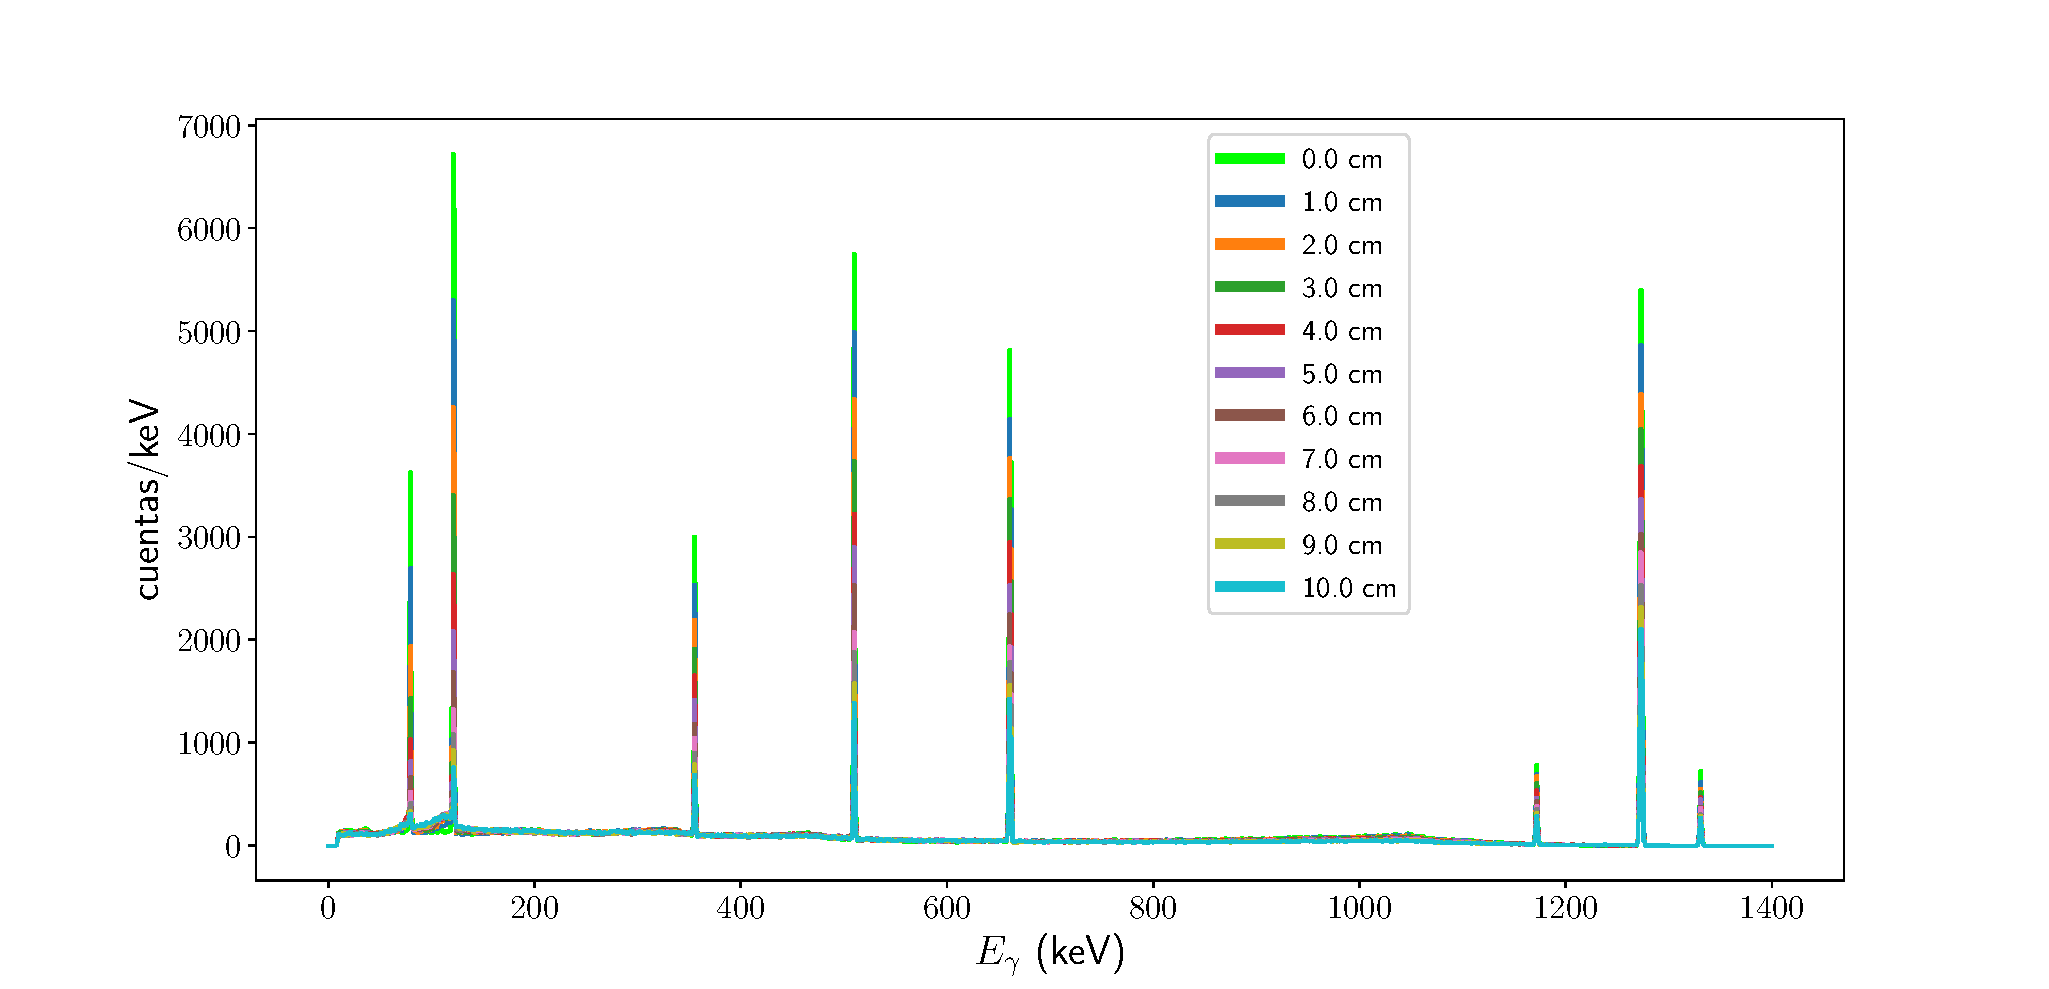
\includegraphics[width=1.0\linewidth]{Kap4/espectro_m1-10M-trans.pdf}
	\caption{Espectro de 10 láminas de Morteros1. Transmisión}
	\label{fig:espectrom1-10m-trans}
\end{figure}


Como se puede ver, cuanto mas grueso el material, la intensidad máxima disminuye. Esto se debe a que obedece la ecuación \ref{intensidad}. 

\begin{equation}\label{intensidad}
	I=I_0e^{-\mu x}
\end{equation}

donde $I_0$ es la intensidad inicial, $\mu$ el coeficiente de atenuación y $x$ el grosor del material. Esta ultima es la variable, en el presente texto será llamada $t$. El valor de $\mu$ es encontrado para cada fotopico. Es fácil ver que se tendrán 8 valores. Con estos se hace un ajuste de la forma:

\begin{equation}
	\frac{\mu}{\rho}=\alpha\times E^{-n}.
\end{equation}

\begin{figure}[H]
	\centering
	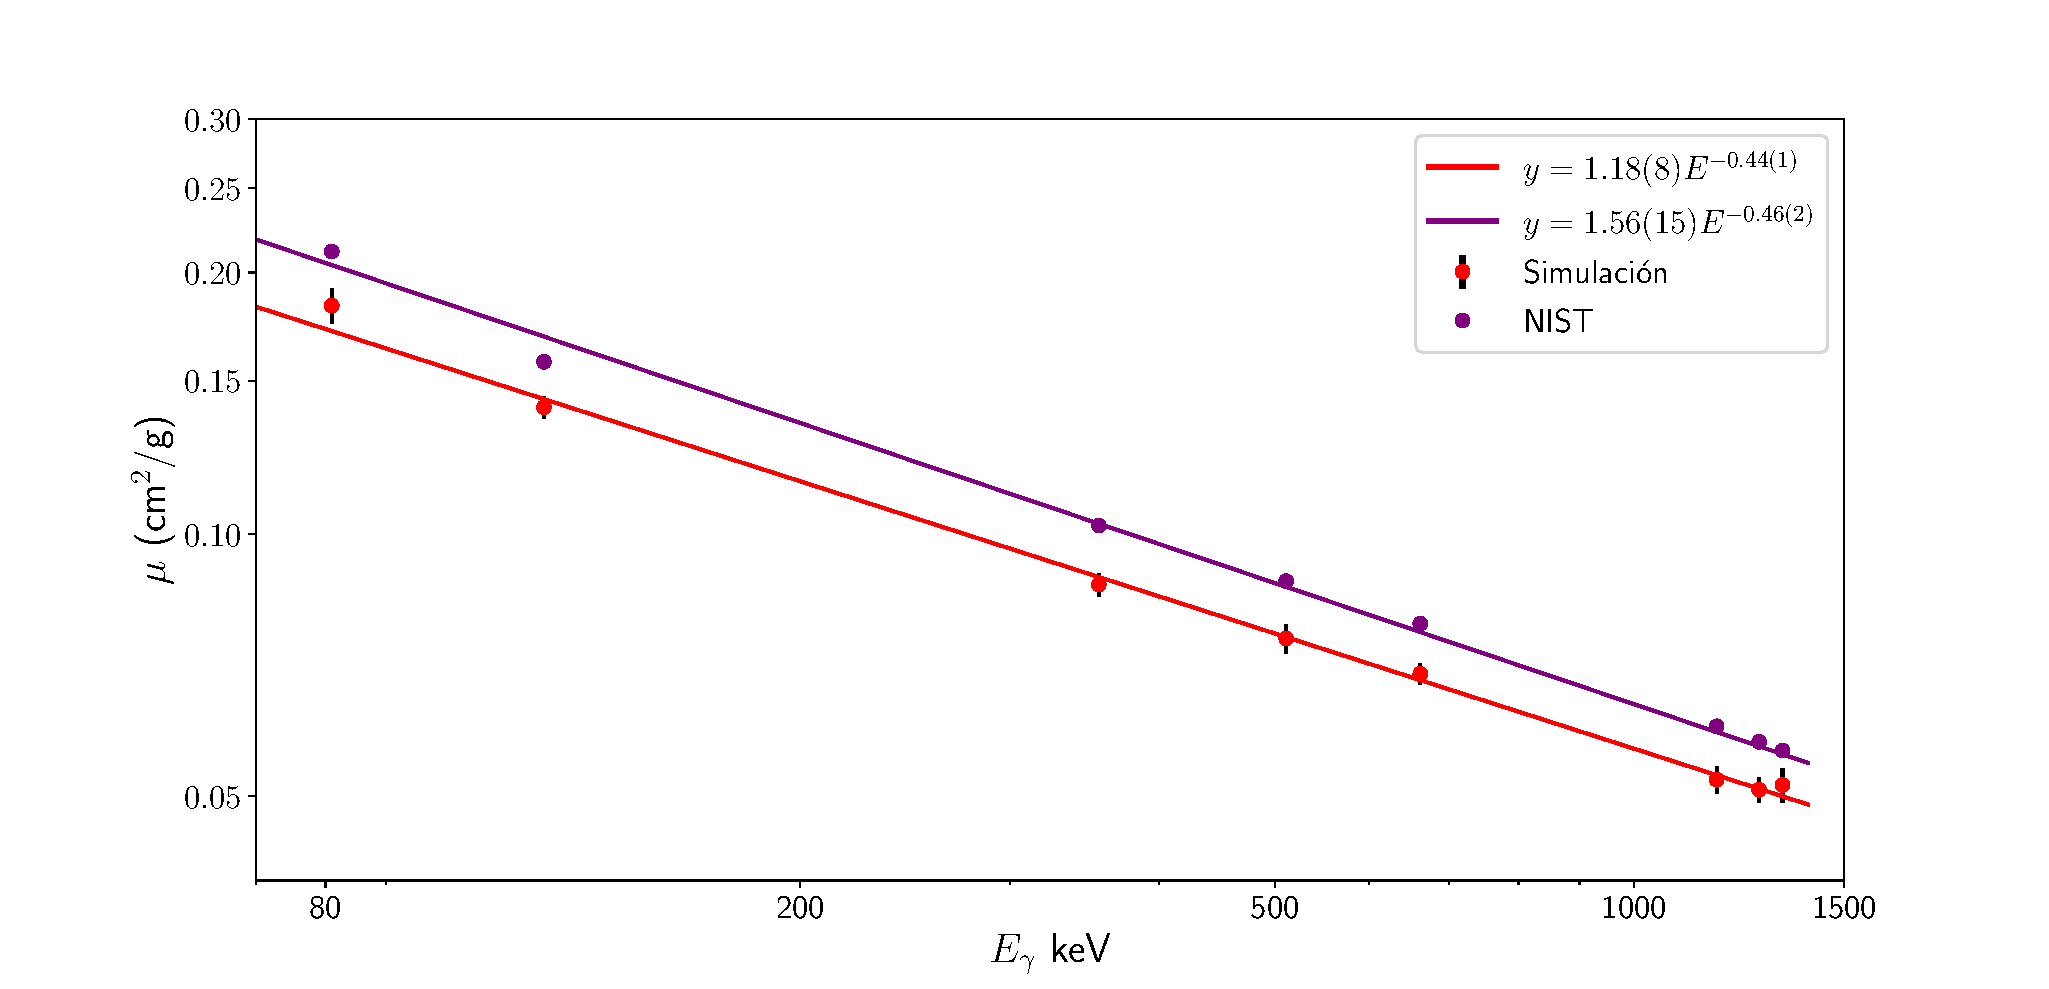
\includegraphics[width=1.0\linewidth]{Kap4/mu-trans-m1.pdf}
	\caption{Ajuste para encontrar $\alpha$ y $n$ a partir de los diferentes $\mu$/$\rho$. Morteros1.}
	\label{fig:mu-trans-m1}
\end{figure}

En la figura anterior podemos ver los valores de interés con su respectiva incertidumbre. Es importante mencionar que allí se grafica el coeficiente de atenuación másico $\mu_T$, el cual fue definido anteriormente. Como se puede observar, los resultados obtenidos con la simulación son similares a los de la base de datos NIST. Por otro lado, la incertidumbre para los datos de NIST esta asociada unicamente al ajuste.

 
\subsection{Retrodispersión.}

\begin{figure}[H]
	\centering
	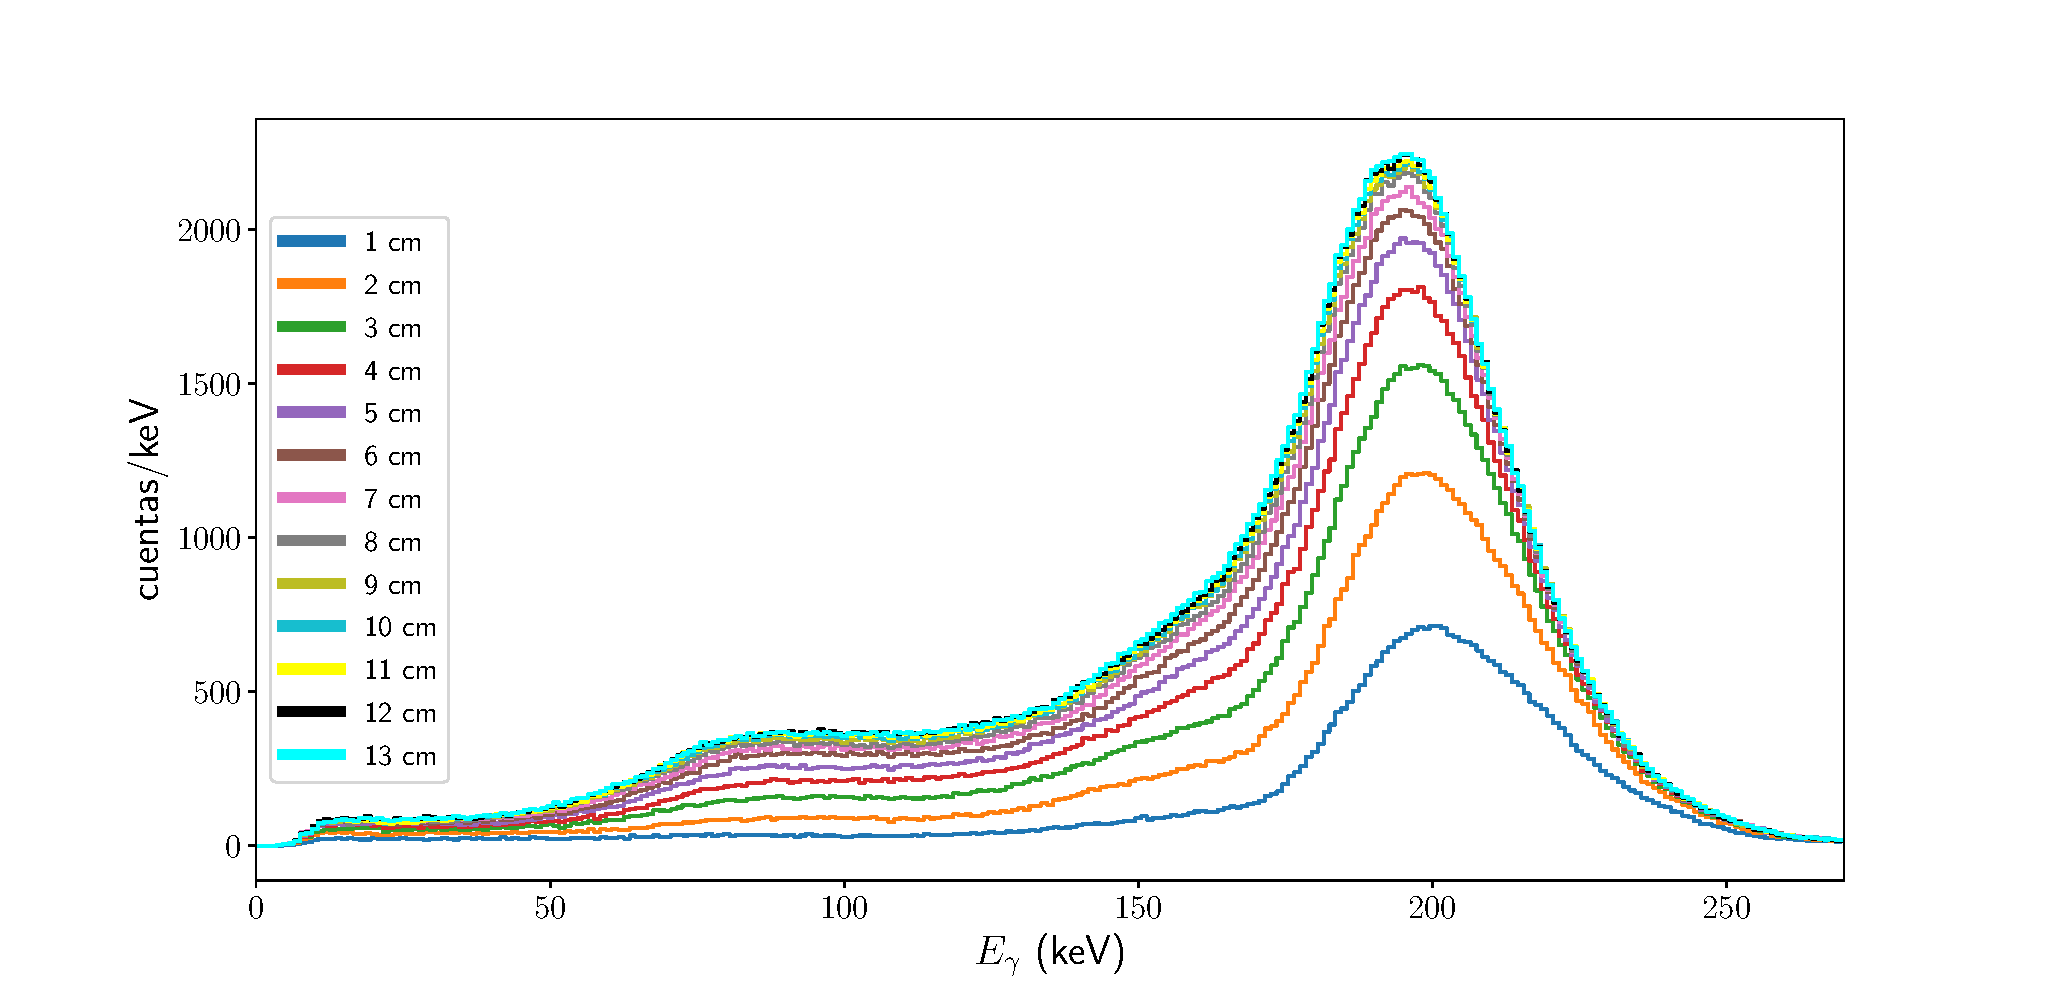
\includegraphics[width=1.0\linewidth]{Kap4/espectros_m1.pdf}
	\caption{Espectro de 10 láminas de Morteros1.}
	\label{fig:espectrosm1}
\end{figure}

En la figura \ref{fig:espectrosm1} se puede apreciar el comportamiento de las intensidades a medida que aumenta el grosor del material. De acuerdo a la figura \ref{g:Montaje-Exp-Retro} los ángulos que abarca la cara del detector mas próxima a las placas son desde $105^\circ$ hasta $164^\circ$, y las energías asociadas son $262$ keV y $197$ keV respectivamente. 
 
\begin{figure}[H]
	\centering
	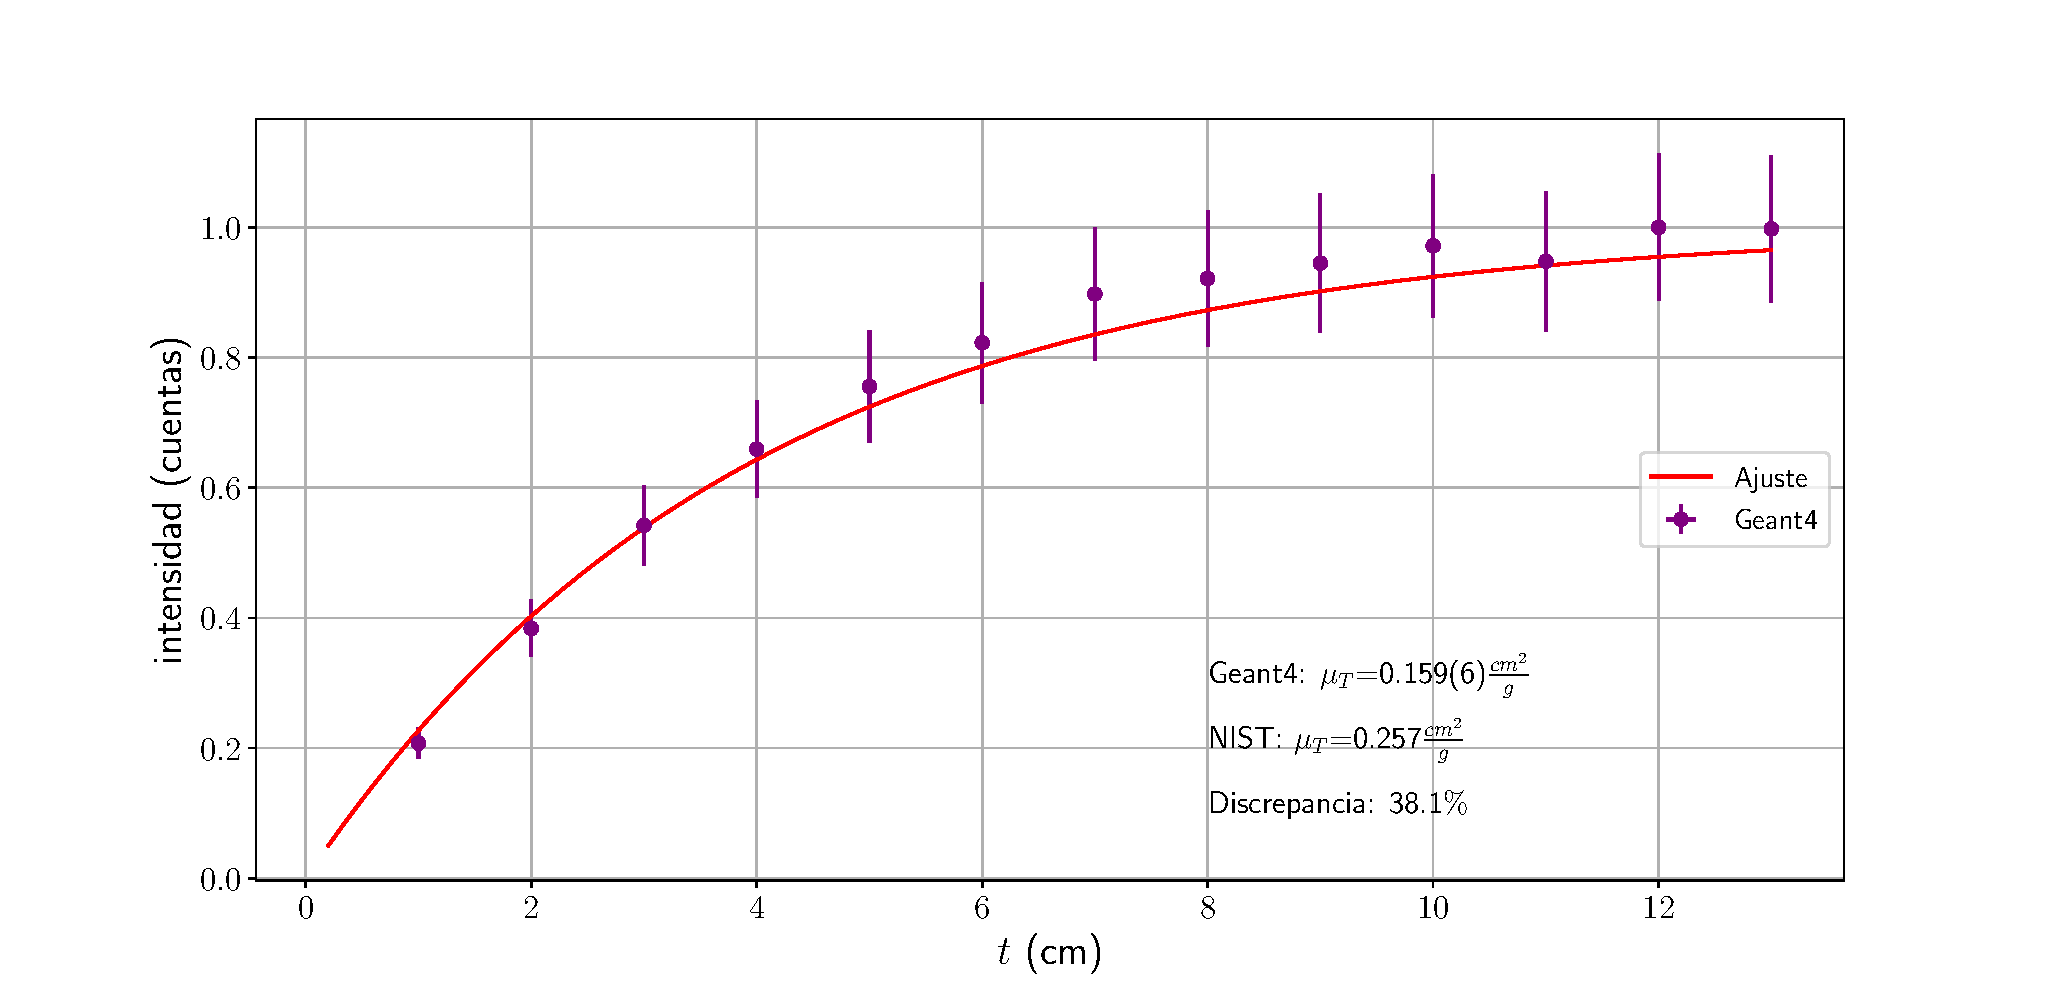
\includegraphics[width=1.0\linewidth]{Kap4/mu_T-m1.pdf}
	\caption{Valores de $\mu_T$ para Morteros 1.}
	\label{fig:mut-m1}
\end{figure}

Una vez encontradas las intensidades asociadas a cada grosor se hace un ajuste tal y como se ve en la figura \ref{fig:mut-m1}. Este ajuste permite encontrar el valor de $\mu_T$, además, de la base de datos NIST se encuentra el valor esta cantidad. Como se puede apreciar, la discrepancia entre estos dos valores es considerable.

 \section{Morteros 2.}
 
 En la tabla \ref{t:medidas-morteros2} se encuentran las dimensiones asociadas a los morteros de este lote. Es importante mencionar que dichos valores son similares con respecto al lote anterior, pues en ambos casos se usaron los mismos recipientes para la construcción.
 
 
 \begin{table}[H]
 	\centering
 	\begin{tabular}{|c|c|c|c|c|c|c|c|}
 		\hline
 		\multicolumn{8}{|c|}{Laminas de Morteros2}                                                                             \\ \hline
 		\multirow{2}{*}{Lamina \#} & Masa {[}g{]} & H1 {[}cm{]} & H2 {[}cm{]} & L1 {[}cm{]} & L2 {[}cm{]} & W1 {[}cm{]} & W2 {[}cm{]} \\ \cline{2-8} 
 		& (+/- 0.01)   & \multicolumn{6}{c|}{(+/- 0.001)}                                                  \\ \hline
 		1                          & 149.35       & 9.760       & 9.706      &9.518         & 9.523      & 0.757       & 0.974       \\ \hline
 		2                          & 157.36       & 9.742       & 9.753      &9.564         & 9.624      & 0.955       & 0.991       \\ \hline
 		3                          & 151.53       & 9.742       & 9.722      &9.615         & 9.493      & 0.923       & 0.956       \\ \hline
 		4                          & 136.97       & 9.757       & 9.794      &9.577         & 9.528      & 0.871       & 0.921       \\ \hline
 	\end{tabular}
 	\caption{Medidas experimentales del lote morteros2.}
 	\label{t:medidas-morteros2}
 \end{table}
 
 En la tabla \ref{t:materiales-mor2} se observa la composición.
 
 \begin{table}[H]
 	\centering
 	\begin{tabular}{|c|c|c|}
 		\hline
 		\multirow{2}{*}{Material} & \multicolumn{2}{c|}{4 placas} \\ \cline{2-3}
 		& g         	& \%        	\\ \hline
 		Cemento Portland      	& 160      	& 22.535    	\\ \hline
 		Arena Peña         	& 450      	& 63.380    	\\ \hline
 		Agua                  	& 100     	& 14.084     	\\ \hline
 	\end{tabular}
 	\caption{Proporción porcentual en la elaboración de morteros2.}
 	\label{t:materiales-morteros2}
 \end{table}
 
 Se evidencia que la densidad no cambia mucho respecto al anterior lote, esto se debe a que la composición es similar.
 
 \begin{equation} \label{densidad-mor2}
 \rho=\frac{masa}{volumen}=1.75(5) g/cm^3
 \end{equation}
 
 \subsection{Transmisión.}
 
\begin{figure}[H]
	\centering
	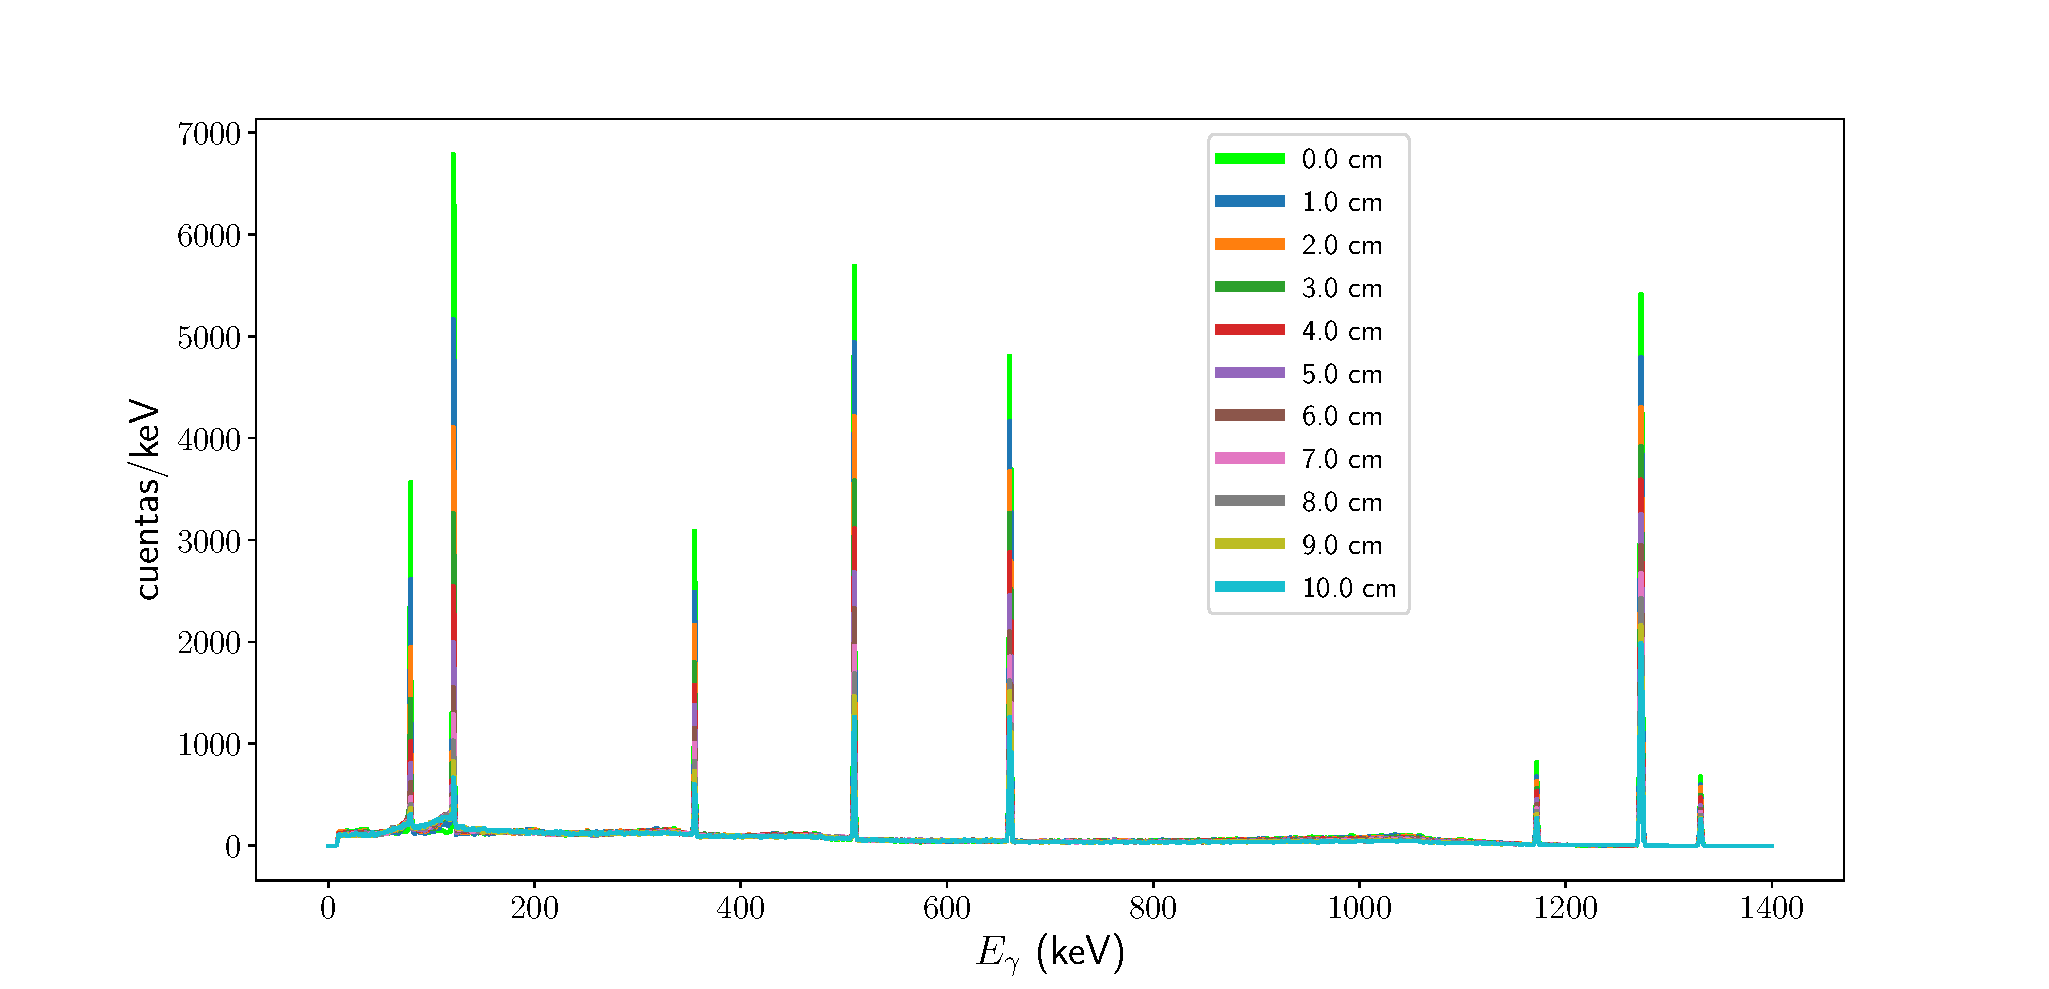
\includegraphics[width=1.0\linewidth]{Kap4/espectro_m2-10M-trans.pdf}
	\caption{Espectro de 10 láminas de Morteros2. Transmisión.}
	\label{fig:espectrom2-10m-trans}
\end{figure}
 
 
\begin{figure}[H]
	\centering
	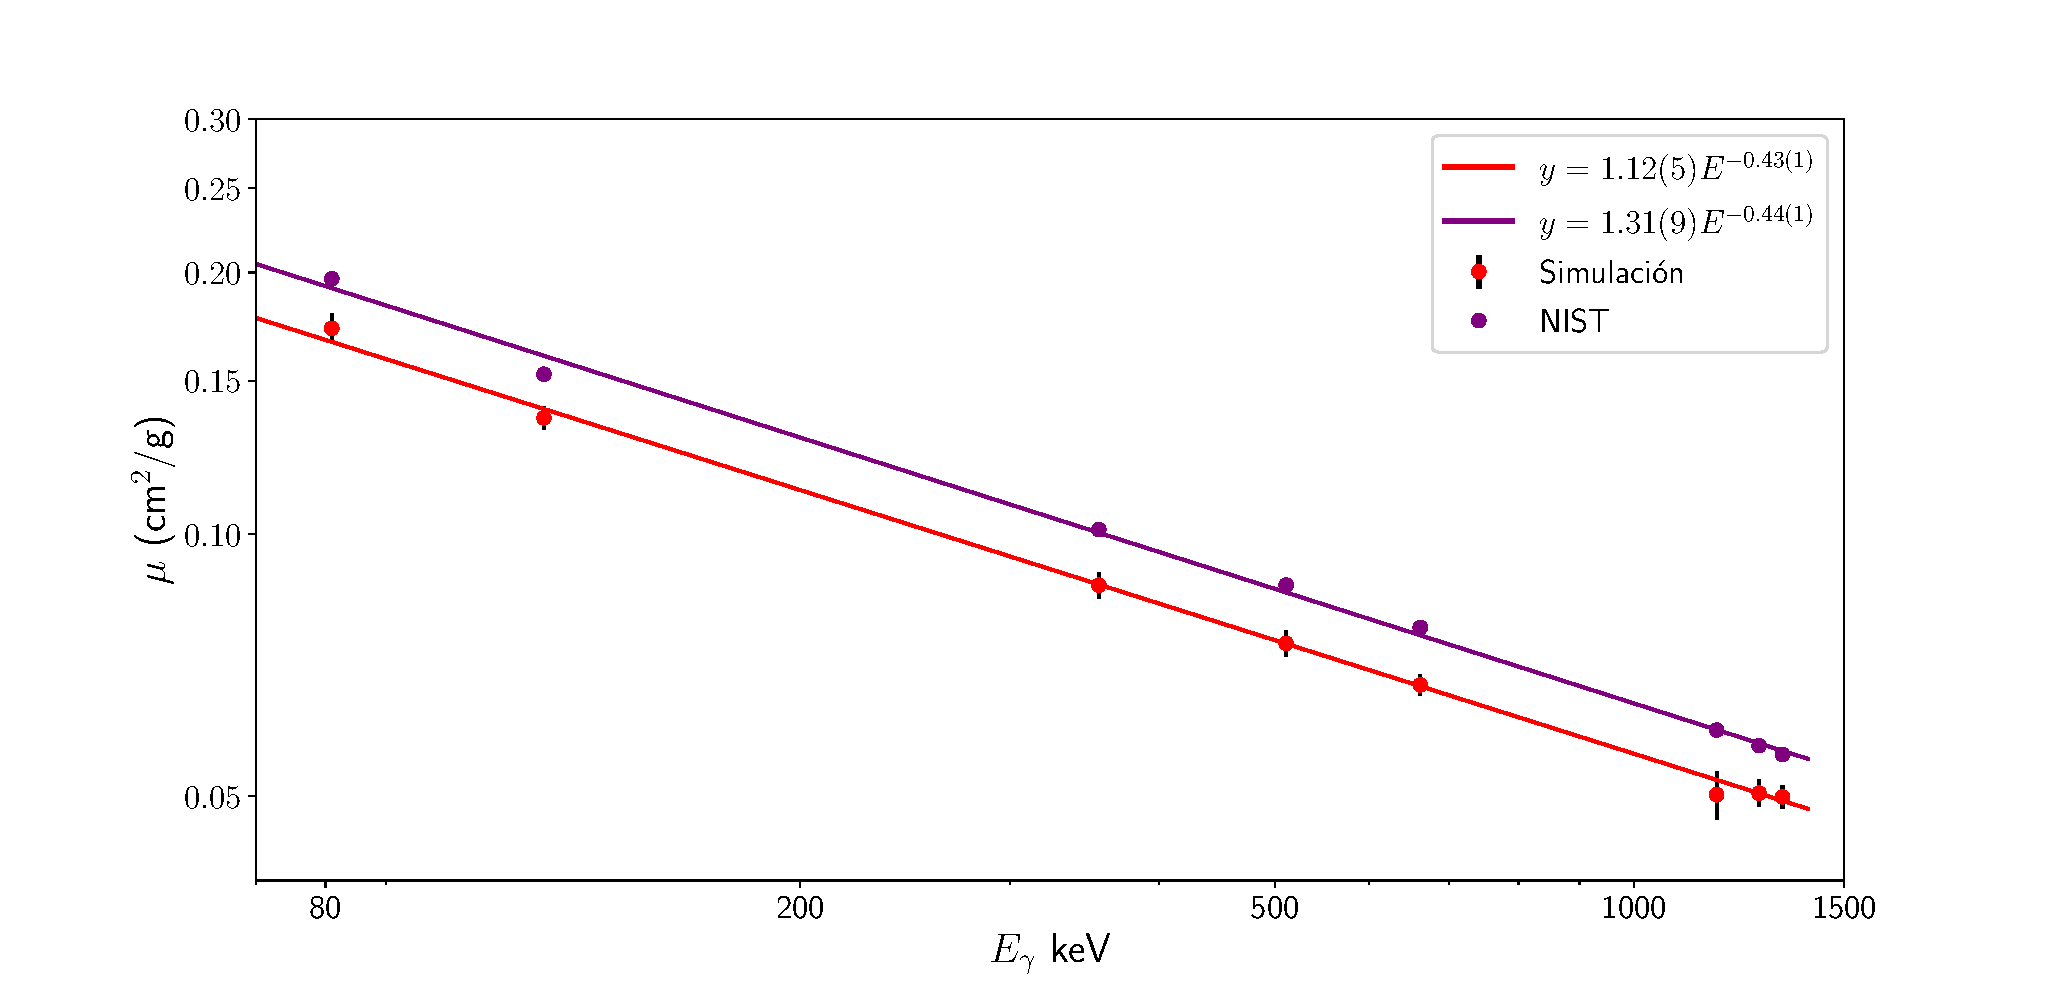
\includegraphics[width=1.0\linewidth]{Kap4/mu-trans-m2.pdf}
	\caption{Ajuste para encontrar $\alpha$ y $n$ a partir de los diferentes $\mu$/$\rho$. Morteros2.}
	\label{fig:mu-trans-m2}
\end{figure}
 
 
 \subsection{Retrodispersión.}
 
 
\begin{figure}[H]
	\centering
	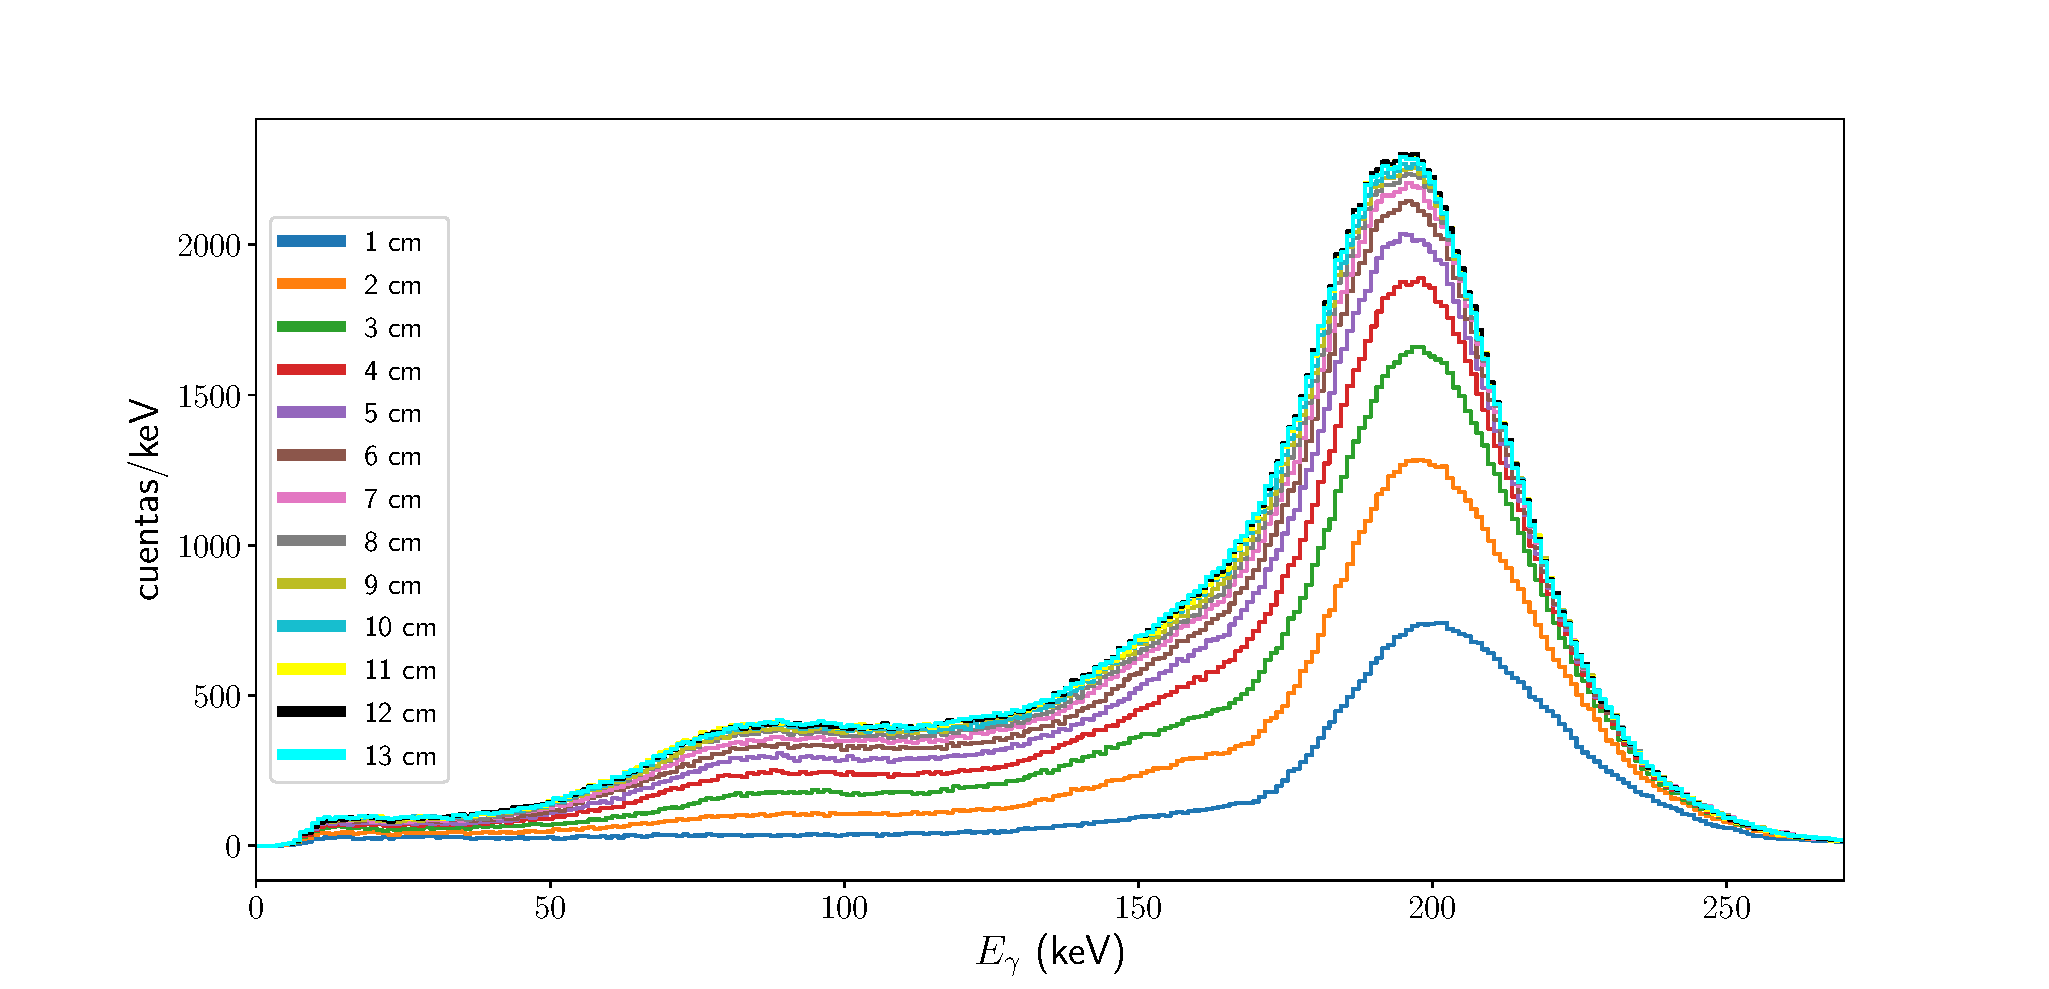
\includegraphics[width=1.0\linewidth]{Kap4/espectro_m2.pdf}
	\caption{Espectro de 10 láminas de Morteros1.}
	\label{fig:espectrom2}
\end{figure}
 
\begin{figure}[H]
	\centering
	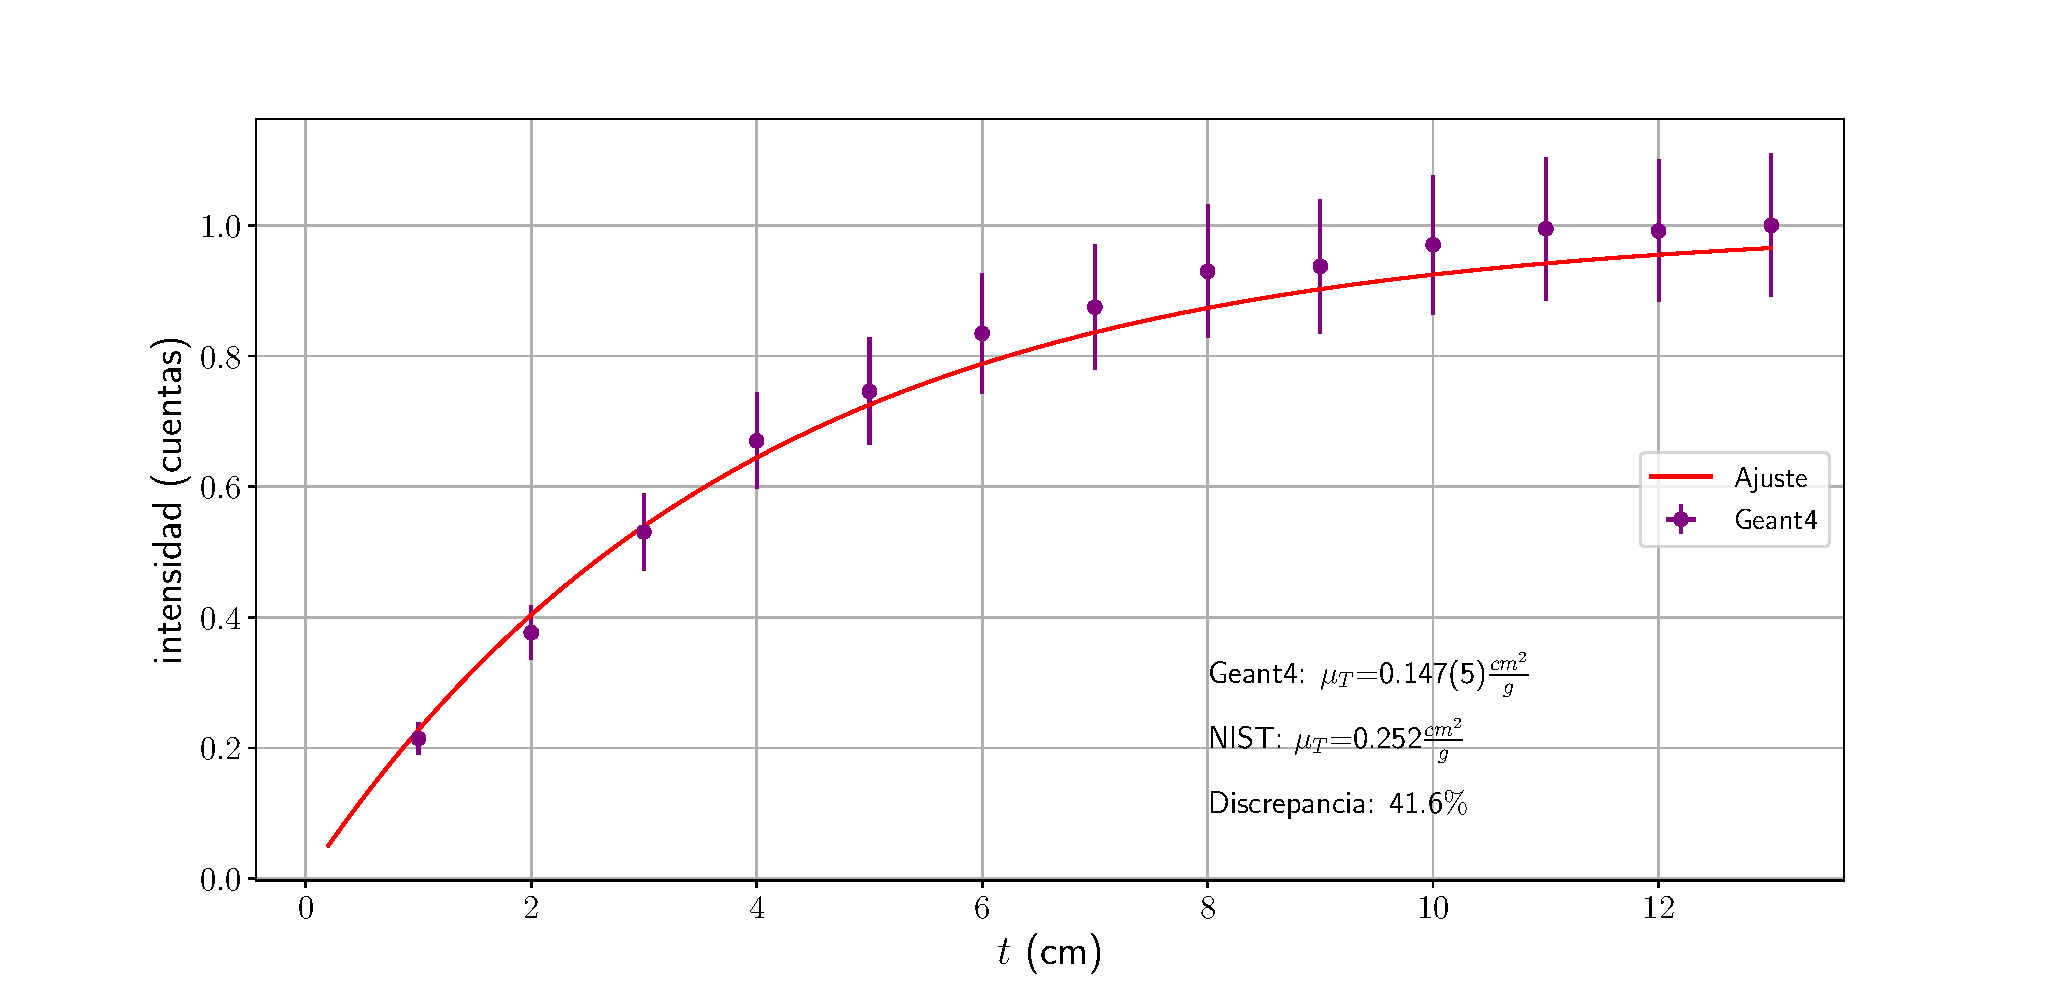
\includegraphics[width=1.0\linewidth]{Kap4/mu_T-m2.pdf}
	\caption{Valores para $\mu_T$. Morteros2.}
	\label{fig:mut-m2}
\end{figure}
 
 
 
 \section{Morteros 3.}
 
  \begin{table}[H]
 	\centering
 	\begin{tabular}{|c|c|c|c|c|c|c|c|}
 		\hline
 		\multicolumn{8}{|c|}{Laminas de Morteros3}                                                                             \\ \hline
 		\multirow{2}{*}{Lamina \#} & Masa {[}g{]} & H1 {[}cm{]} & H2 {[}cm{]} & L1 {[}cm{]} & L2 {[}cm{]} & W1 {[}cm{]} & W2 {[}cm{]} \\ \cline{2-8} 
 		& (+/- 0.01)   & \multicolumn{6}{c|}{(+/- 0.001)}                                                  \\ \hline
 		1                          & 148.71       & 9.825        & 9.820      & 9.583         & 9.712      & 0.975       & 0.935       \\ \hline
 		2                          & 150.32       & 9.672        & 9.616      & 9.528         & 9.577      & 0.968       & 0.929       \\ \hline
 		3                          & 139.83       & 9.613        & 9.640      & 9.463         & 9.521      & 0.949       & 0.916       \\ \hline
 		4                          & 133.72       & 9.864        & 9.839      & 9.526         & 9.550      & 0.852       & 0.916       \\ \hline
 	\end{tabular}
 	\caption{Medidas experimentales del lote morteros2.}
 	\label{t:medidas-morteros3}
 \end{table}
 
 
 \begin{table}[H]
 	\centering
 	\begin{tabular}{|c|c|c|}
 		\hline
 		\multirow{2}{*}{Material} & \multicolumn{2}{c|}{4 placas} \\ \cline{2-3}
 		& g         	& \%        	\\ \hline
 		Cemento Portland      	& 110      	& 15.492    	\\ \hline
 		Arena Sílice         	& 500      	& 70.422    	\\ \hline
 		Agua                  	& 100     	& 14.084     	\\ \hline
 	\end{tabular}
 	\caption{Proporción porcentual en la elaboración de morteros2.}
 	\label{t:materiales-morteros3}
 \end{table}
 
 \begin{equation} \label{densidad-mor3}
 \rho=\frac{masa}{volumen}=1.62(7) g/cm^3
 \end{equation}
 
 \subsection{Transmisión.}
 
\begin{figure}[H]
	\centering
	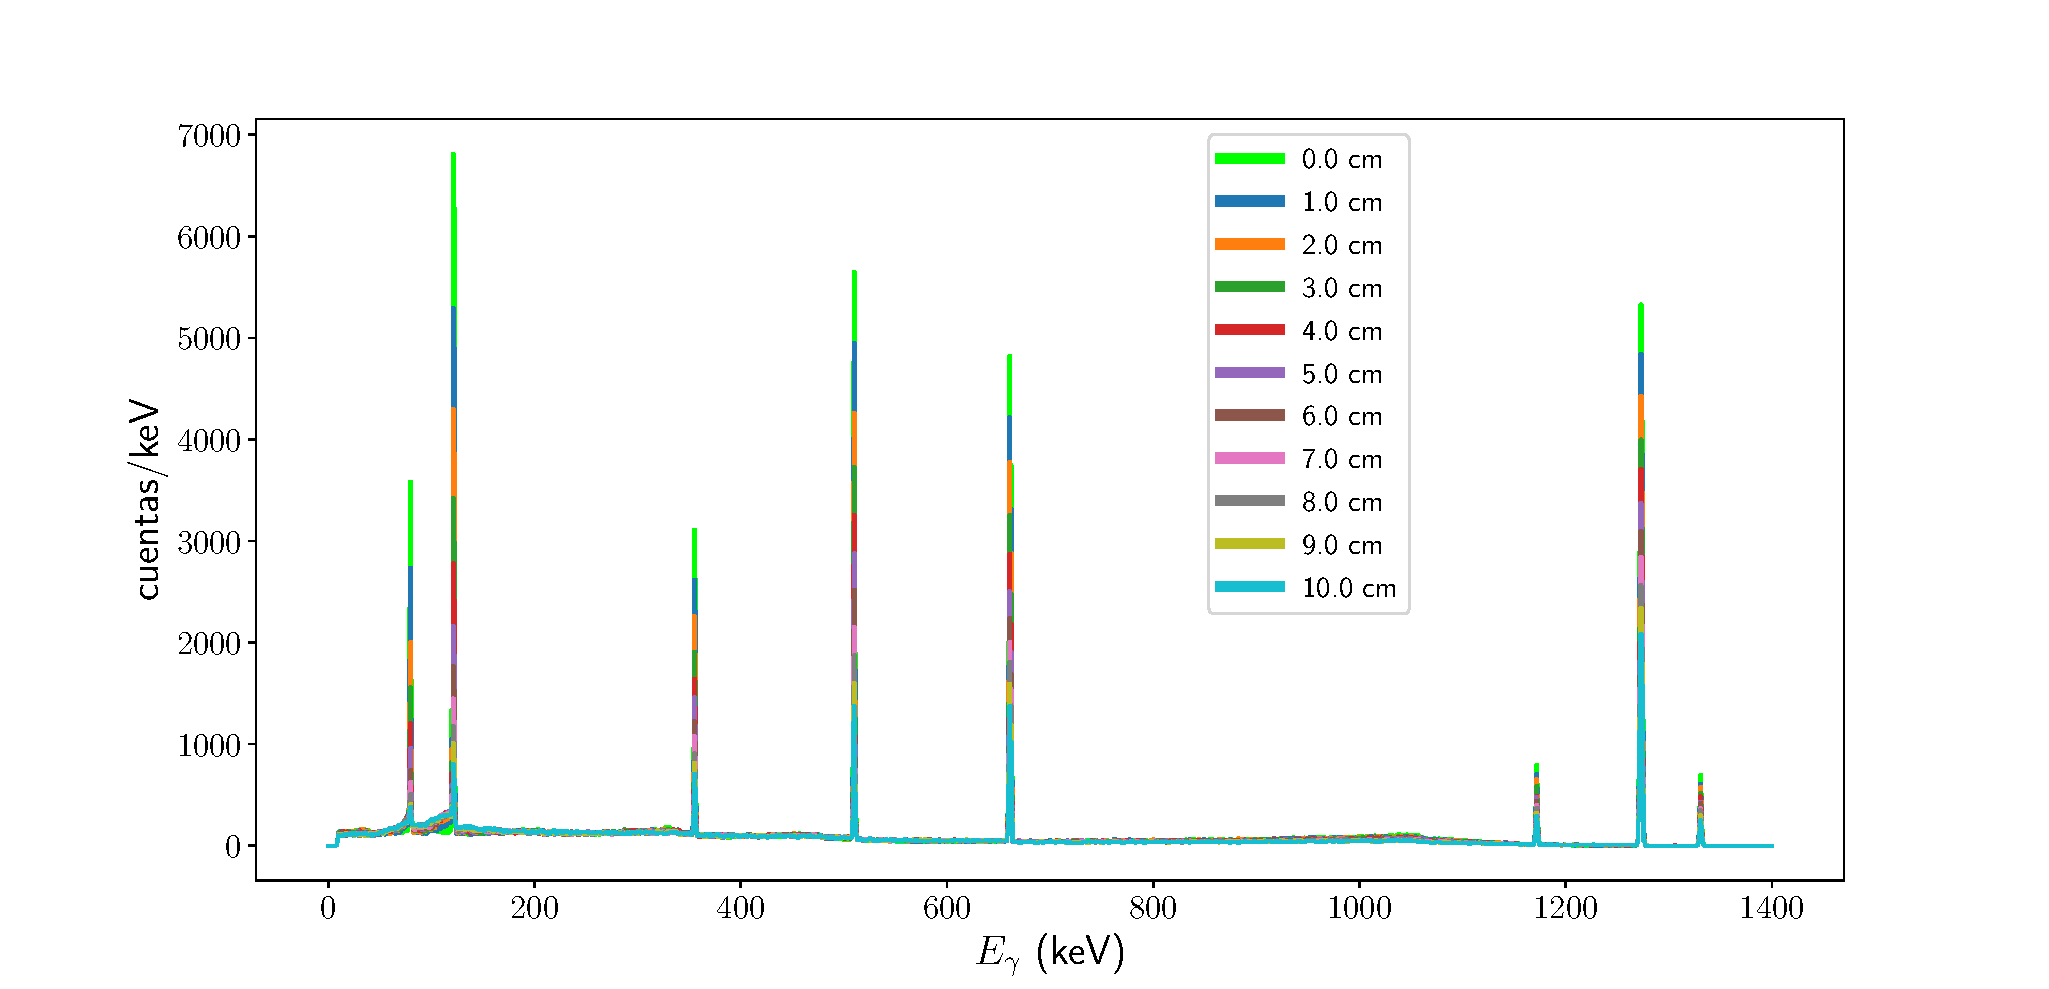
\includegraphics[width=1.0\linewidth]{Kap4/espectro_m3-M10-trans.pdf}
	\caption{Espectro de 10 láminas de Morteros3. Transmisión}
	\label{fig:espectrom3-m10-trans}
\end{figure}
 
\begin{figure}[H]
	\centering
	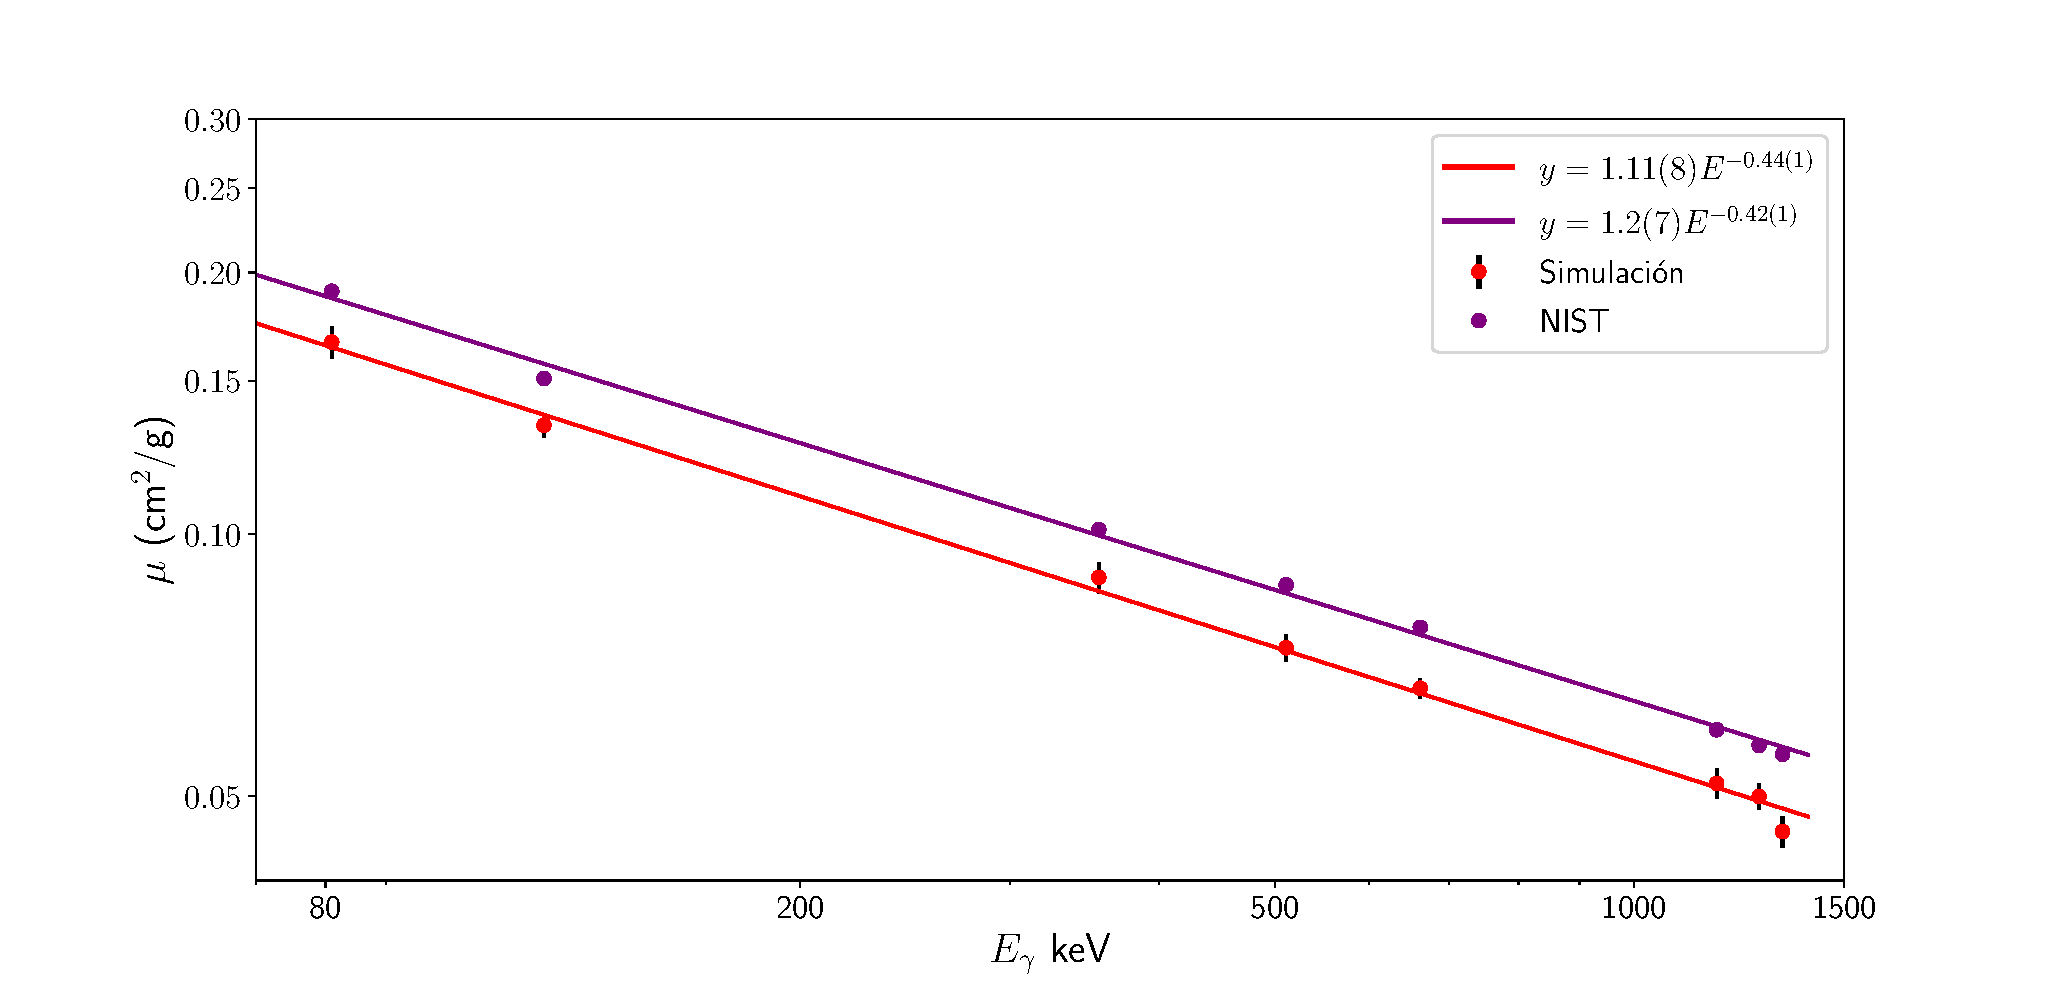
\includegraphics[width=1.0\linewidth]{Kap4/mu-trans-m3.pdf}
	\caption{Ajuste para encontrar $\alpha$ y $n$ a partir de los diferentes $\mu$/$\rho$. Morteros3.}
	\label{fig:mu-trans-m3}
\end{figure}
 
 
 \subsection{Retrodispersión.}
 
\begin{figure}[H]
	\centering
	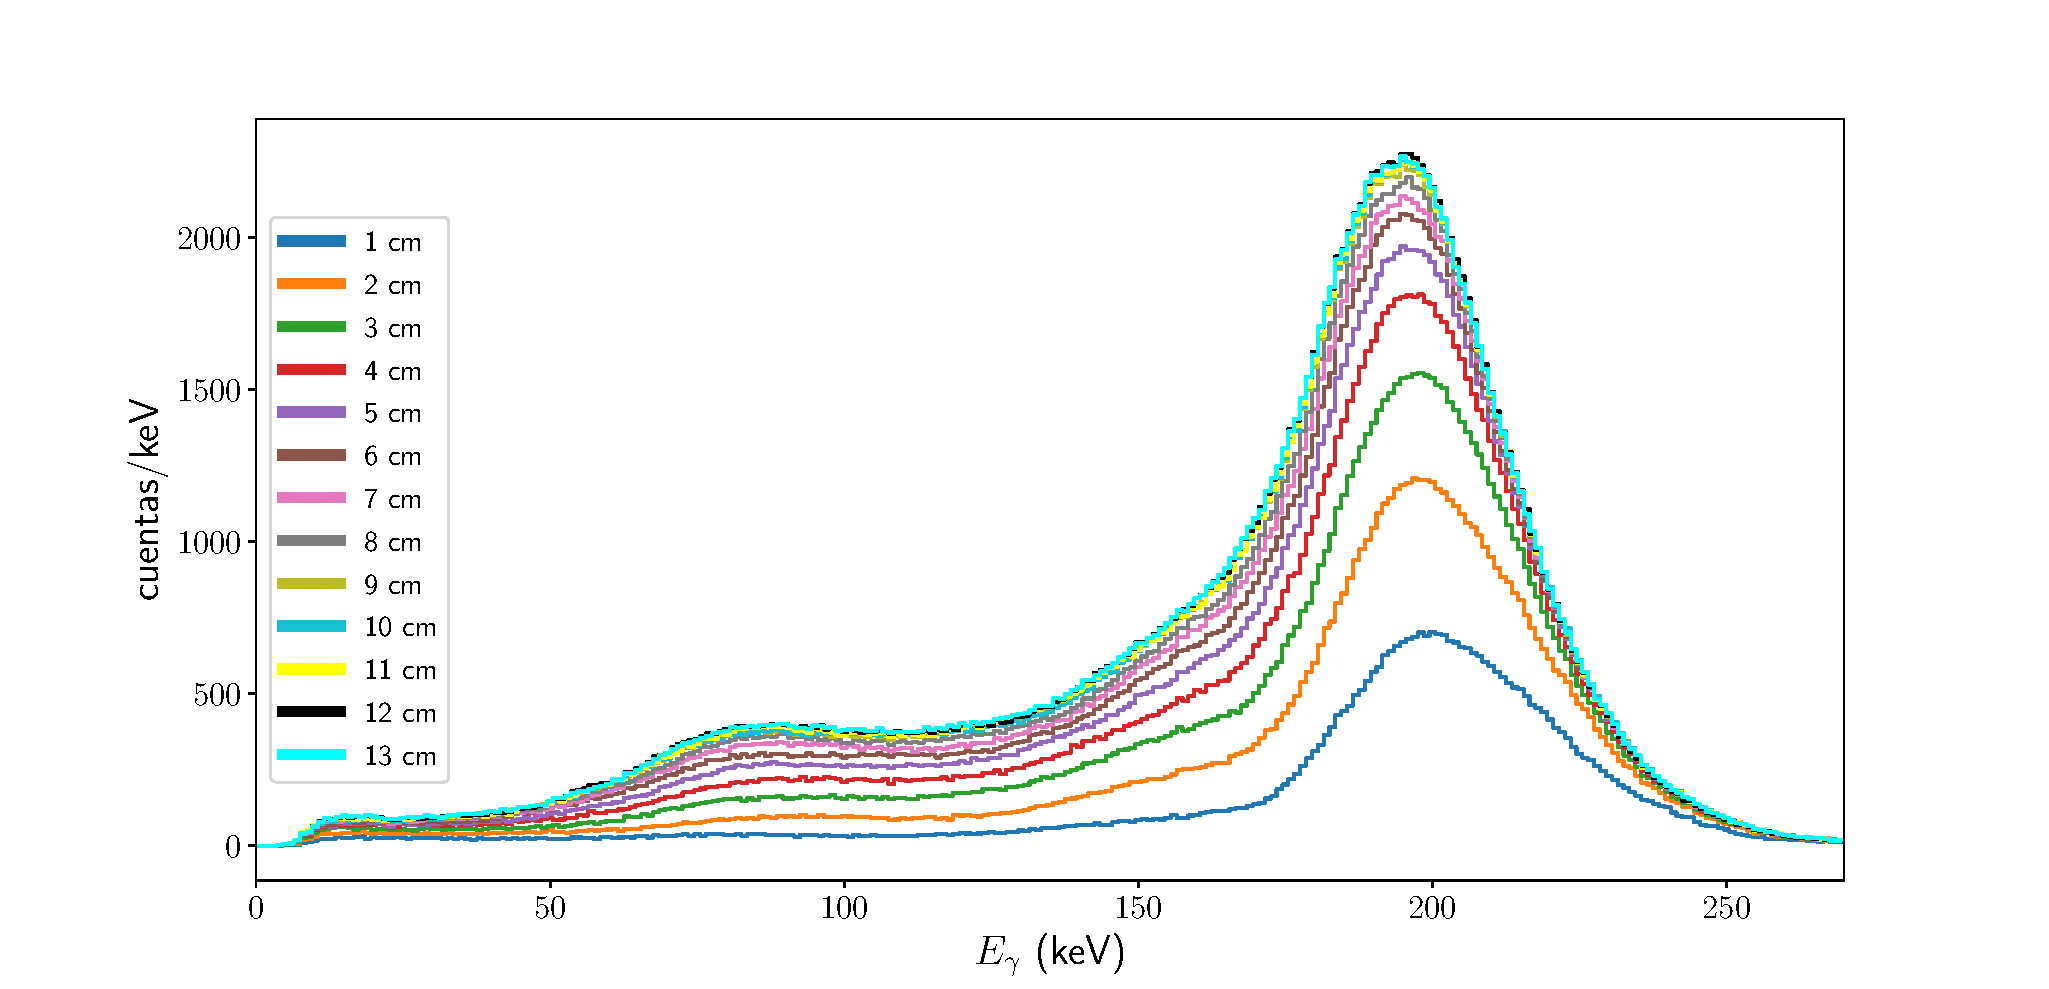
\includegraphics[width=1.0\linewidth]{Kap4/espectro_m3.pdf}
	\caption{Espectro de 10 láminas de Morteros3.}
	\label{fig:espectrom3}
\end{figure}

\begin{figure}[H]
	\centering
	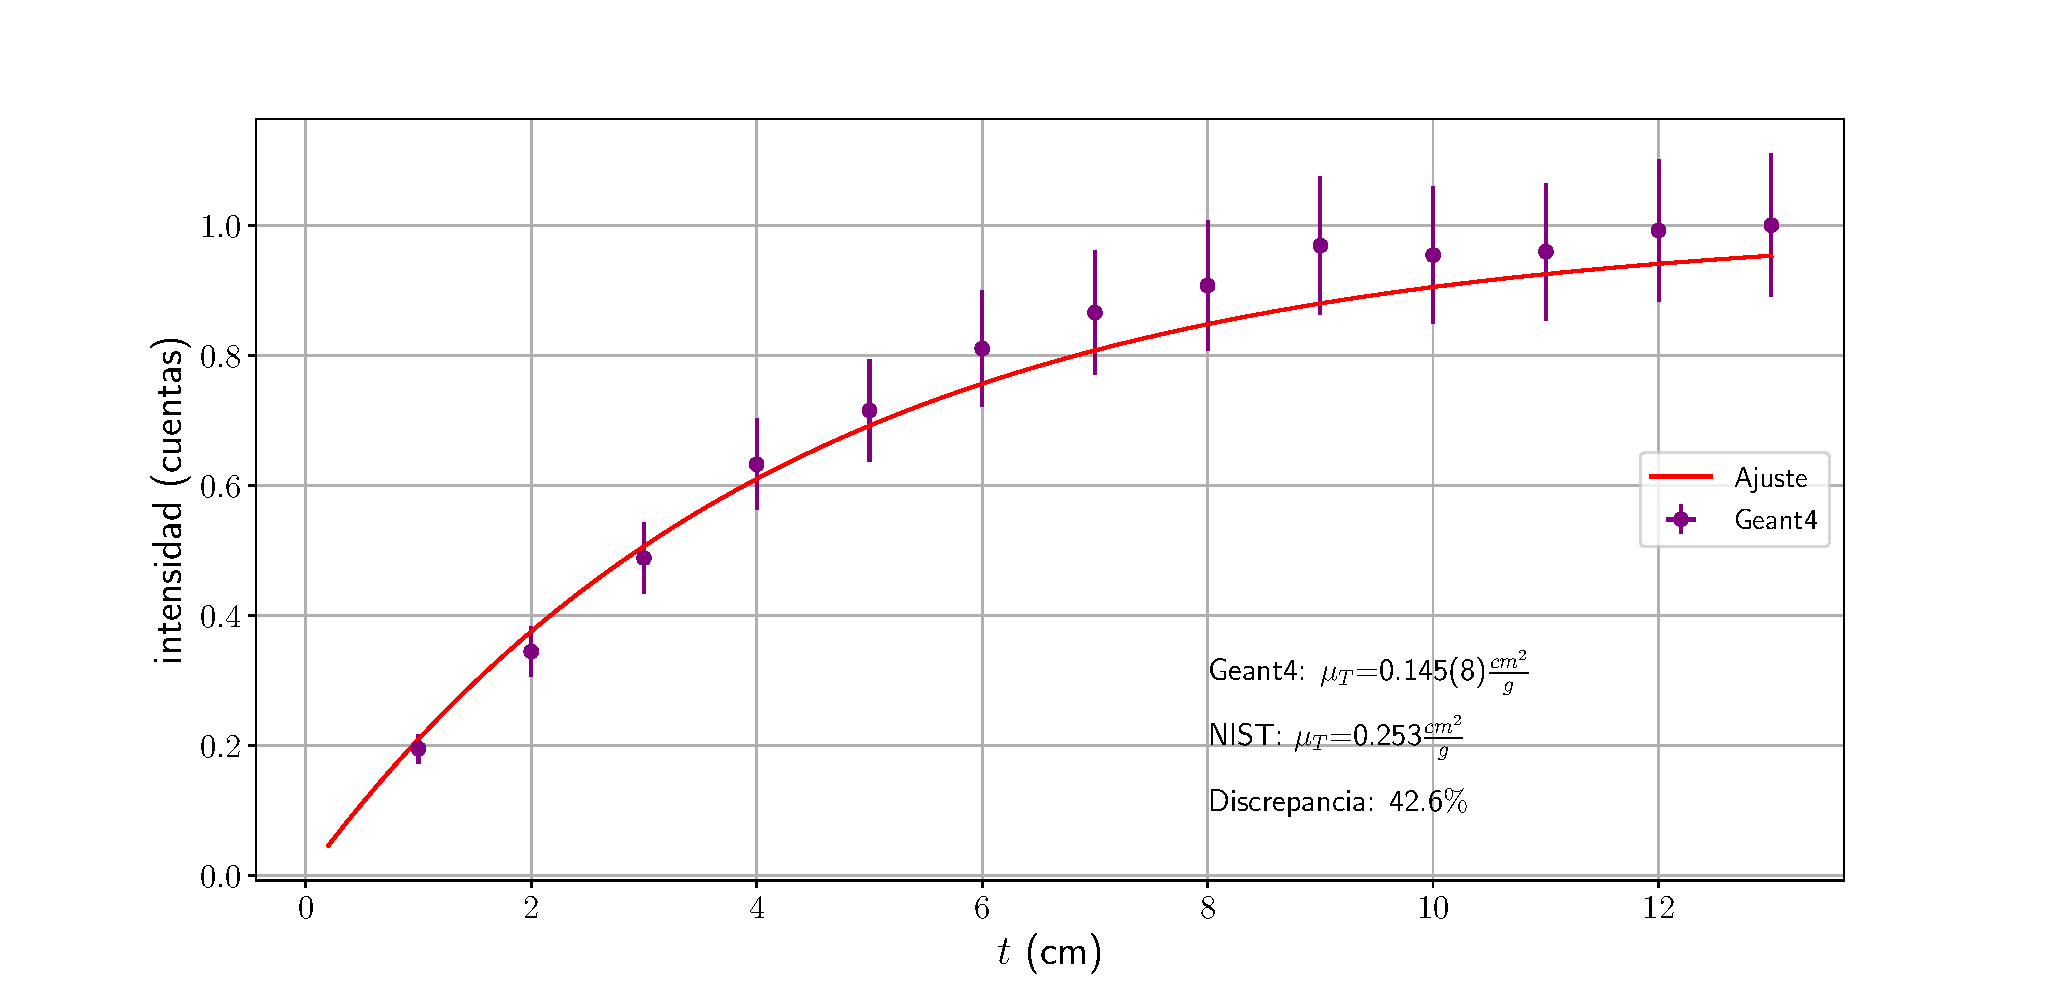
\includegraphics[width=1.0\linewidth]{Kap4/mu_T-m3.pdf}
	\caption{$\mu_T=0.24(1) cm^{-1}$ Morteros3.}
	\label{fig:mut-m3}
\end{figure}

 
 
 
 \section{Morteros 4.}
 
   \begin{table}[H]
 	\centering
 	\begin{tabular}{|c|c|c|c|c|c|c|c|}
 		\hline
 		\multicolumn{8}{|c|}{Laminas de Morteros4}                                                                             \\ \hline
 		\multirow{Lamina \#} & Masa {[}g{]} & H1 {[}cm{]} & H2 {[}cm{]} & L1 {[}cm{]} & L2 {[}cm{]} & W1 {[}cm{]} & W2 {[}cm{]} \\ \cline{2-8} 
 		& (+/- 0.01)   & \multicolumn{6}{c|}{(+/- 0.001)}                                                  \\ \hline
 		1                          & 156.90       & 9.774         & 9.804      & 9.557          & 9.563      & 0.938       & 10.20       \\ \hline
 		2                          & 145.96       & 9.687         & 9.653      & 9.620          & 9.550      & 0.914       & 0.940       \\ \hline
 		3                          & 140.52       & 9.657         & 9.693      & 9.579          & 9.589      & 1.079       & 0.902       \\ \hline
 		4                          & 147.33       & 9.814         & 9.772      & 9.546          & 9.589      & 1.075       & 0.953       \\ \hline
 	\end{tabular}
 	\caption{Medidas experimentales del lote morteros4.}
 	\label{t:medidas-morteros4}
 \end{table}
 
 
 \begin{table}[H]
 	\centering
 	\begin{tabular}{|c|c|c|}
 		\hline
 		\multirow{Material} & \multicolumn{2}{c|}{4 placas} \\ \cline{2-3}
 		& g         	& \%        	\\ \hline
 		Cemento Portland      	& 100      	& 10.989    	\\ \hline
 		Arena Sílice         	& 700      	& 76.923    	\\ \hline
 		Agua                  	& 110     	& 12.087     	\\ \hline
 	\end{tabular}
 	\caption{Proporción porcentual en la elaboración de morteros4.}
 	\label{t:materiales-morteros4}
 \end{table}
 
 \begin{equation} \label{densidad-mor4}
 \rho=\frac{masa}{volumen}=1.62(3) g/cm^3
 \end{equation}
 
 \subsection{Transmisión.}
 
\begin{figure}[H]
	\centering
	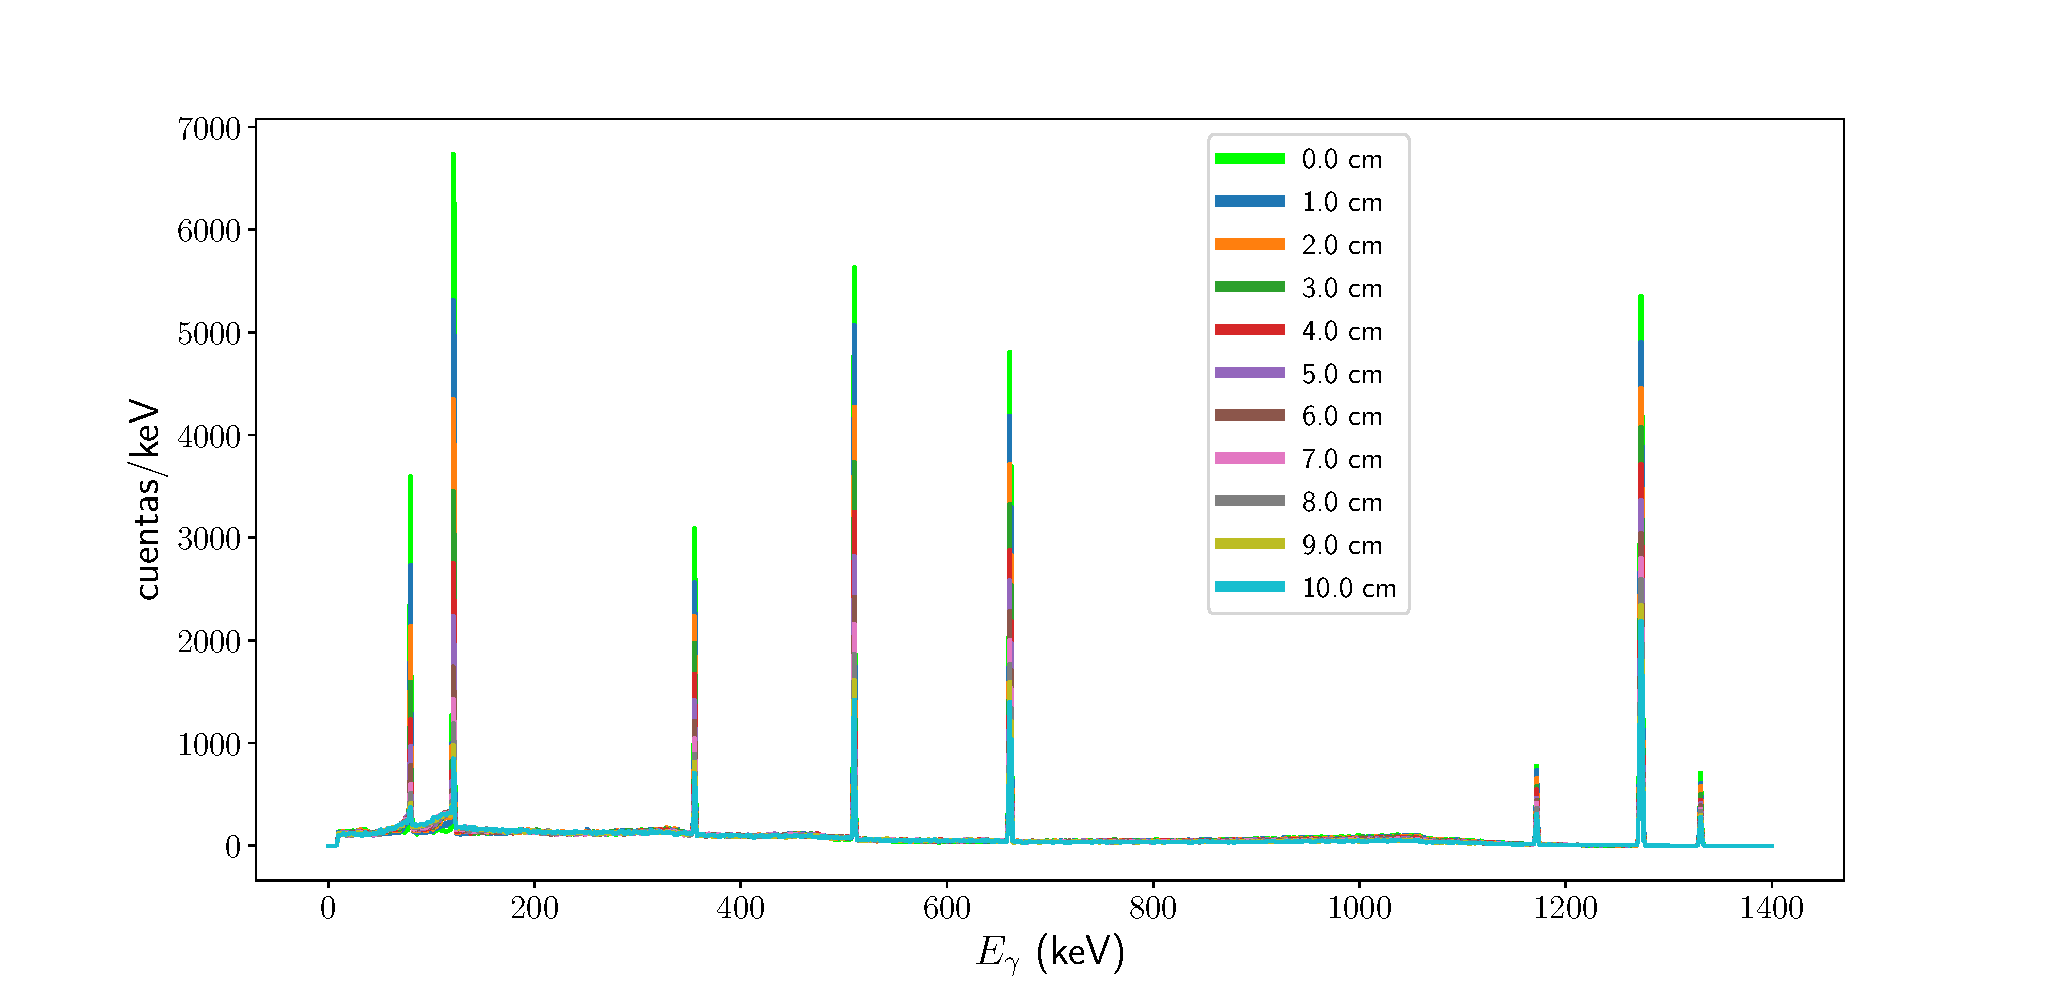
\includegraphics[width=1.0\linewidth]{Kap4/espectro_m4-10M-trans.pdf}
	\caption{Espectro de 10 láminas de Morteros4. Transmisicón}
	\label{fig:espectrom4-10m-trans}
\end{figure}
 
\begin{figure}[H]
	\centering
	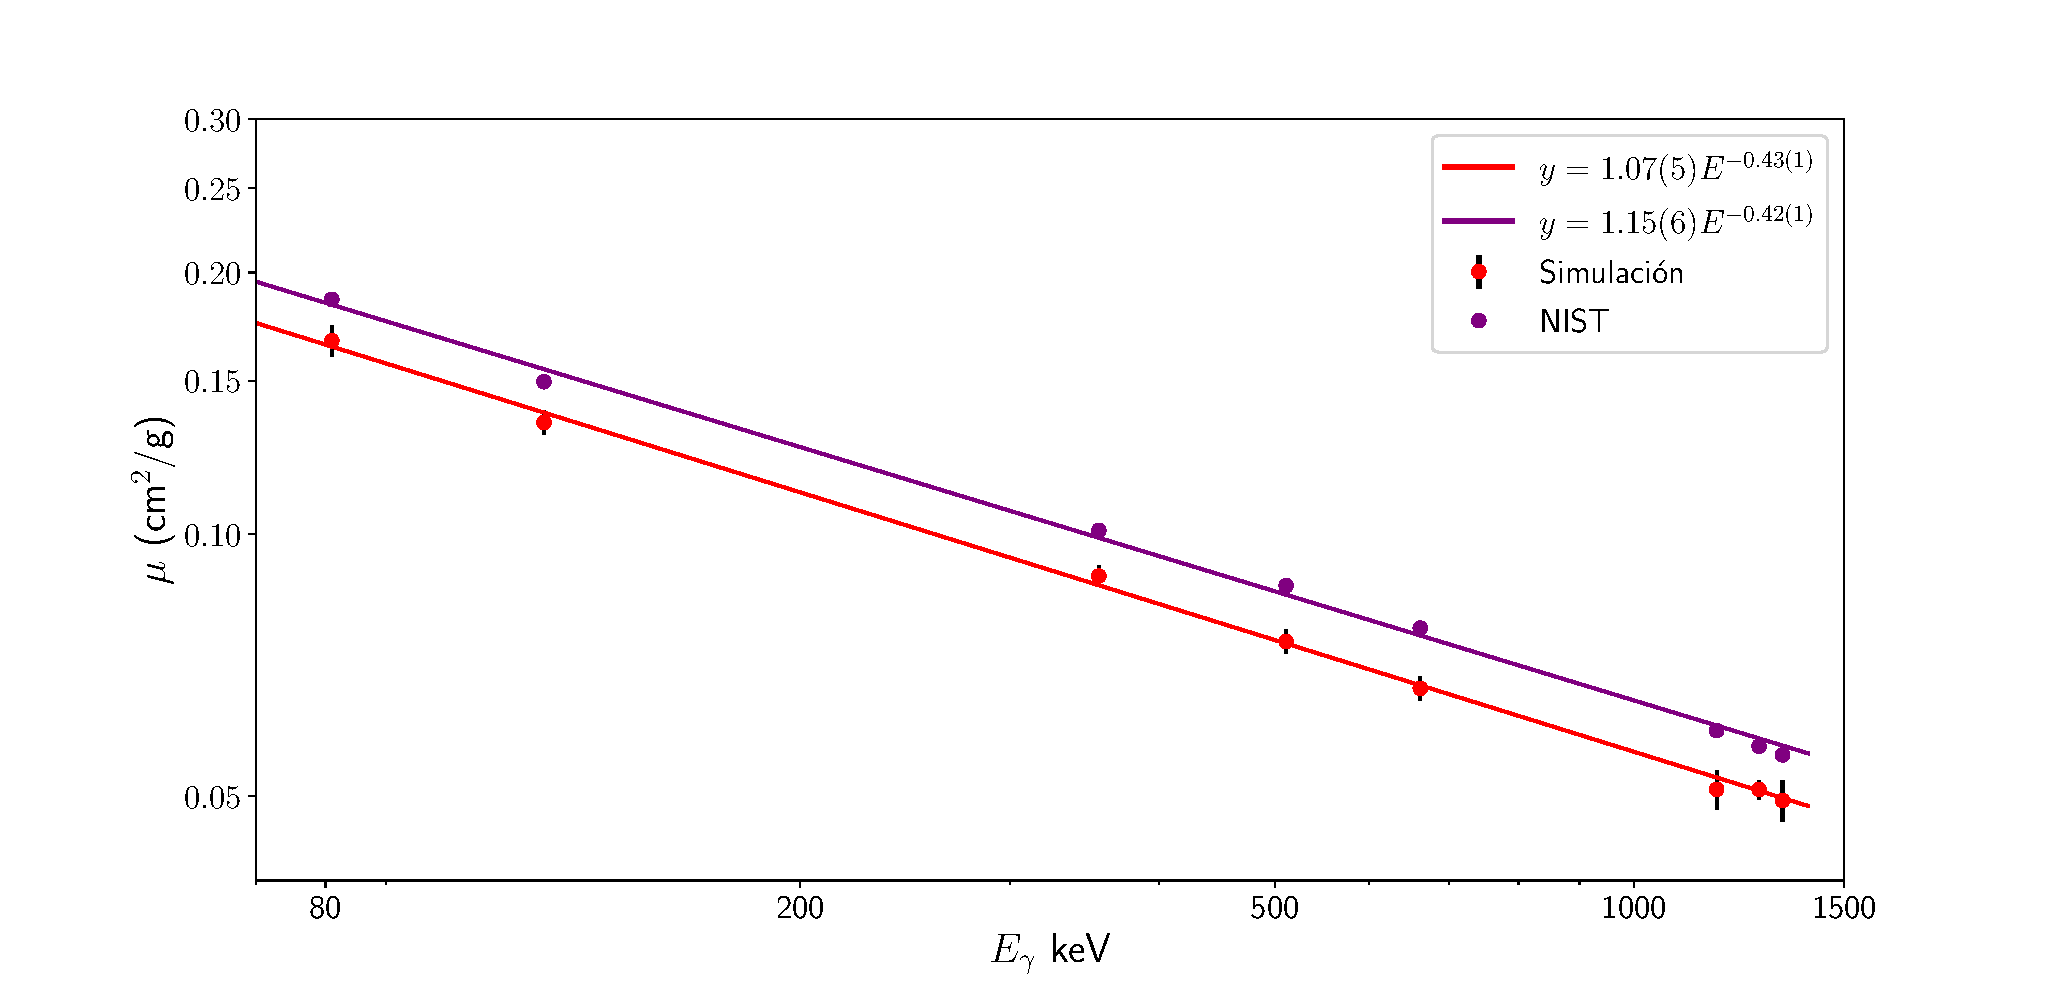
\includegraphics[width=1.0\linewidth]{Kap4/mu-trans-m4.pdf}
	\caption{Ajuste para encontrar $\alpha$ y $n$ a partir de los diferentes $\mu$/$\rho$. Morteros4.}
	\label{fig:mu-trans-m4}
\end{figure}
 
 
 \subsection{Retrodispersión.}
 
 \begin{figure}[H]
 	\centering
 	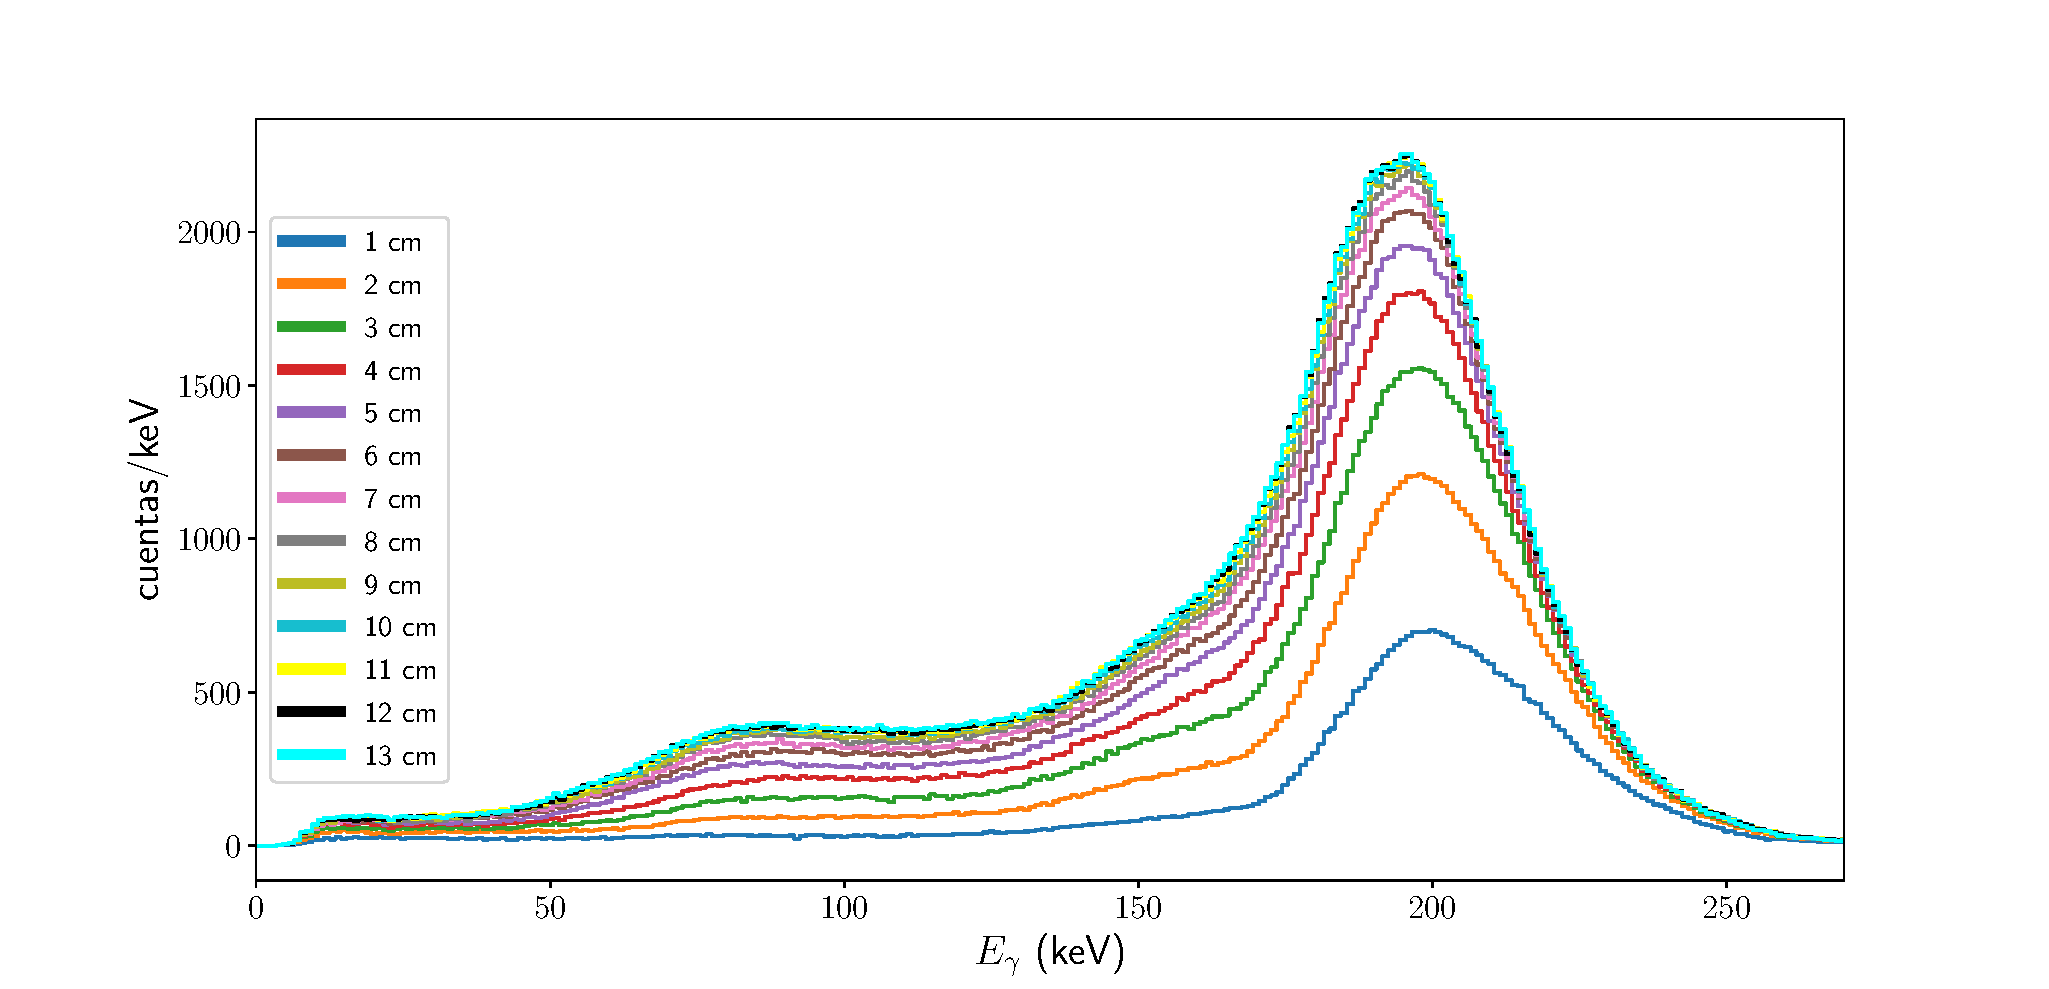
\includegraphics[width=1.0\linewidth]{Kap4/espectro_m4.pdf}
 	\caption{Espectro de 10 láminas de Morteros4.}
 	\label{fig:espectrom4}
 \end{figure}
 
 \begin{figure}[H]
 	\centering
 	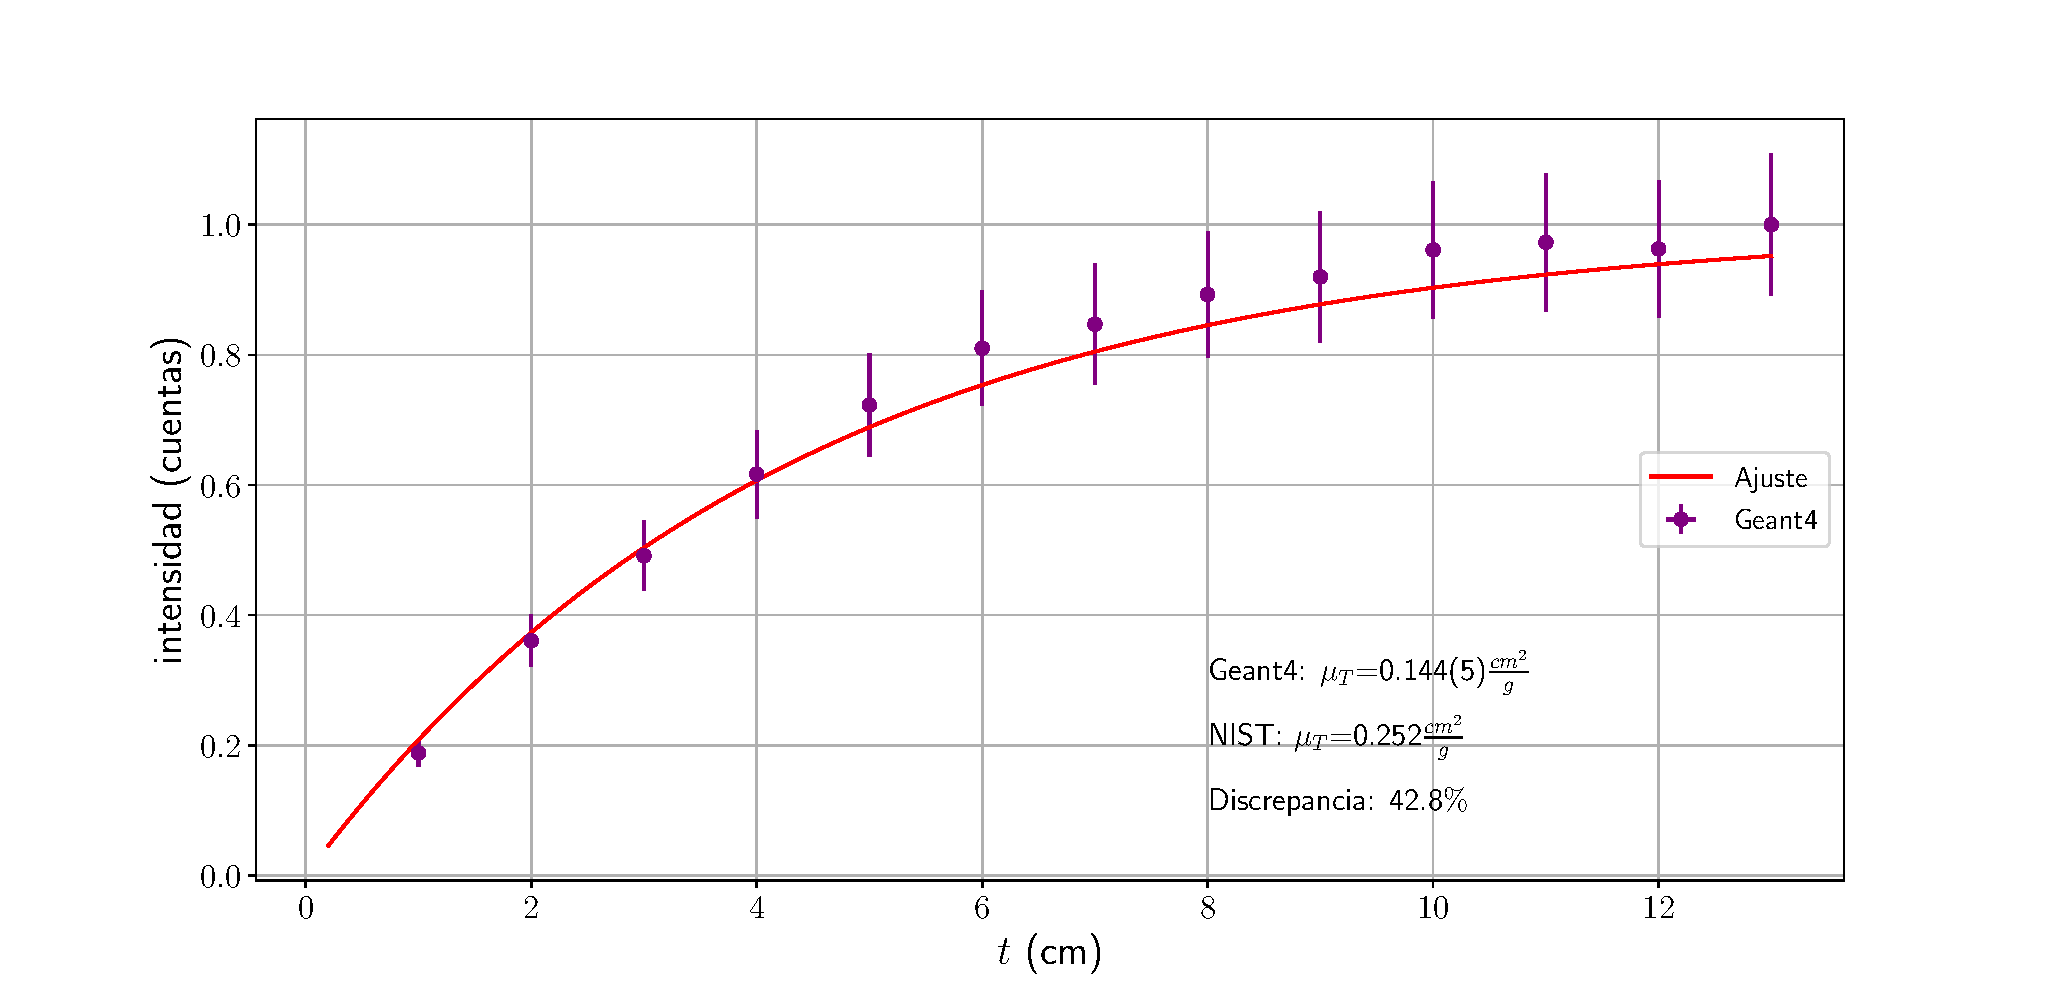
\includegraphics[width=1.0\linewidth]{Kap4/mu_T-m4.pdf}
 	\caption{valores de $\mu_T$. Morteros4.}
 	\label{fig:mut-m4}
 \end{figure}
 
 
 
 
 \section{Morteros 5.}
 
    \begin{table}[H]
 	\centering
 	\begin{tabular}{|c|c|c|c|c|c|c|c|}
 		\hline
 		\multicolumn{8}{|c|}{Laminas de Morteros5}                                                                             \\ \hline
 		\multirow{2}{*}{Lamina \#} & Masa {[}g{]} & H1 {[}cm{]} & H2 {[}cm{]} & L1 {[}cm{]} & L2 {[}cm{]} & W1 {[}cm{]} & W2 {[}cm{]} \\ \cline{2-8} 
 		& (+/- 0.01)   & \multicolumn{6}{c|}{(+/- 0.001)}                                                  \\ \hline 		1                          & 136.58       & 9.762          & 9.734      & 96.67         & 96.10       & 1.009       & 0.877       \\ \hline
 		2                          & 133.28       & 9.660          & 9.646      & 96.00         & 96.42       & 0.850       & 0.887       \\ \hline
 		3                          & 128.12       & 9.629          & 9.673      & 95.11         & 95.30       & 0.927       & 0.824       \\ \hline
 		4                          & 130.35       & 9.670          & 9.677      & 95.77         & 96.93       & 0.869       & 0.912       \\ \hline
 	\end{tabular}
 	\caption{Medidas experimentales del lote morteros5.}
 	\label{t:medidas-morteros5}
 \end{table}
 
 
 \begin{table}[H]
 	\centering
 	\begin{tabular}{|c|c|c|}
 		\hline
 		\multirow{2}{*}{Material} & \multicolumn{2}{c|}{4 placas} \\ \cline{2-3}
 		& g         	& \%        	\\ \hline
 		Cemento Portland      	& 600      	& 75    	\\ \hline
 		Arena Sílice         	& 0      	& 0    	\\ \hline
 		Agua                  	& 200     	& 25     	\\ \hline
 	\end{tabular}
 	\caption{Proporción porcentual en la elaboración de morteros4.}
 	\label{t:materiales-morteros5}
 \end{table}
 
 \begin{equation} \label{densidad-mor5}
 \rho=\frac{masa}{volumen}=1.60(6) g/cm^3
 \end{equation}
 
 
 \subsection{Transmisión.}
 
\begin{figure}[H]
	\centering
	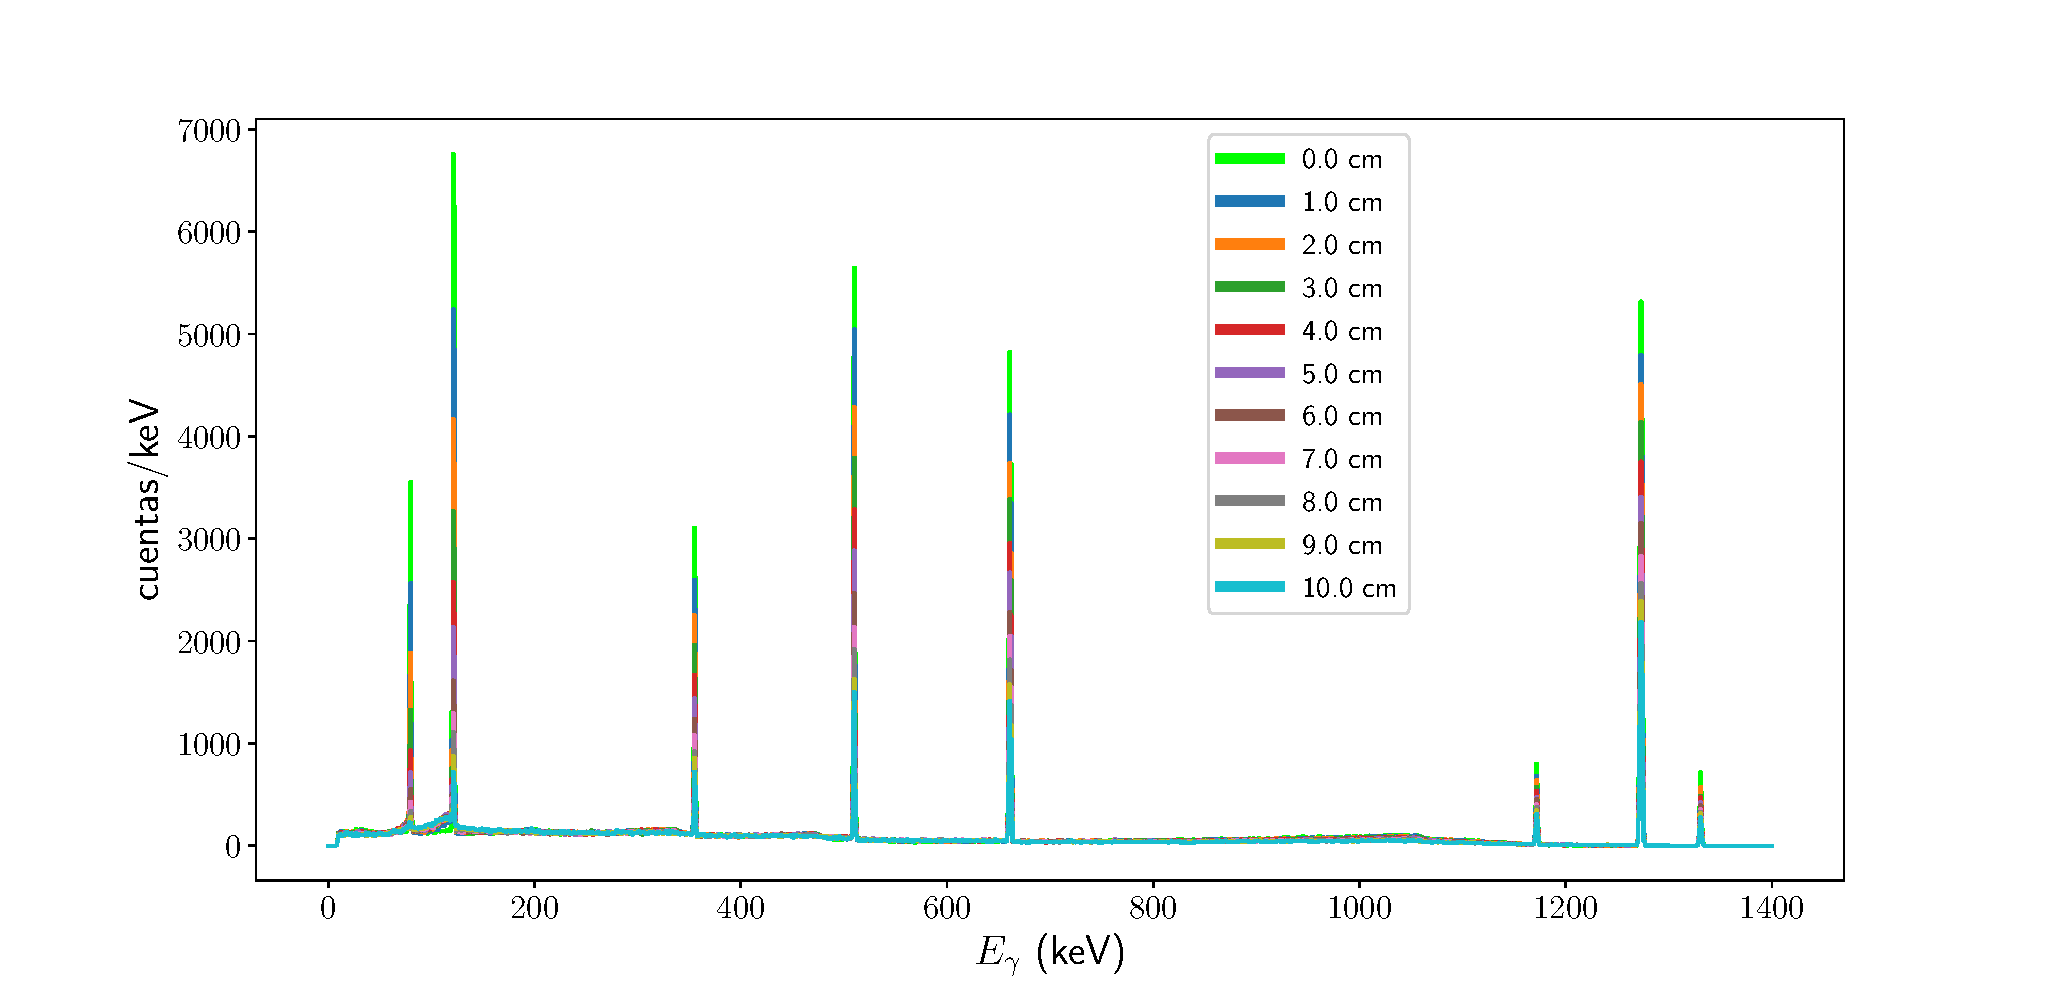
\includegraphics[width=1.0\linewidth]{Kap4/espectro_m5-10Mtrans.pdf}
	\caption{Espectro de 10 láminas de Morteros5. Transmisión}
	\label{fig:espectrom5-10mtrans}
\end{figure}
 
\begin{figure}[H]
	\centering
	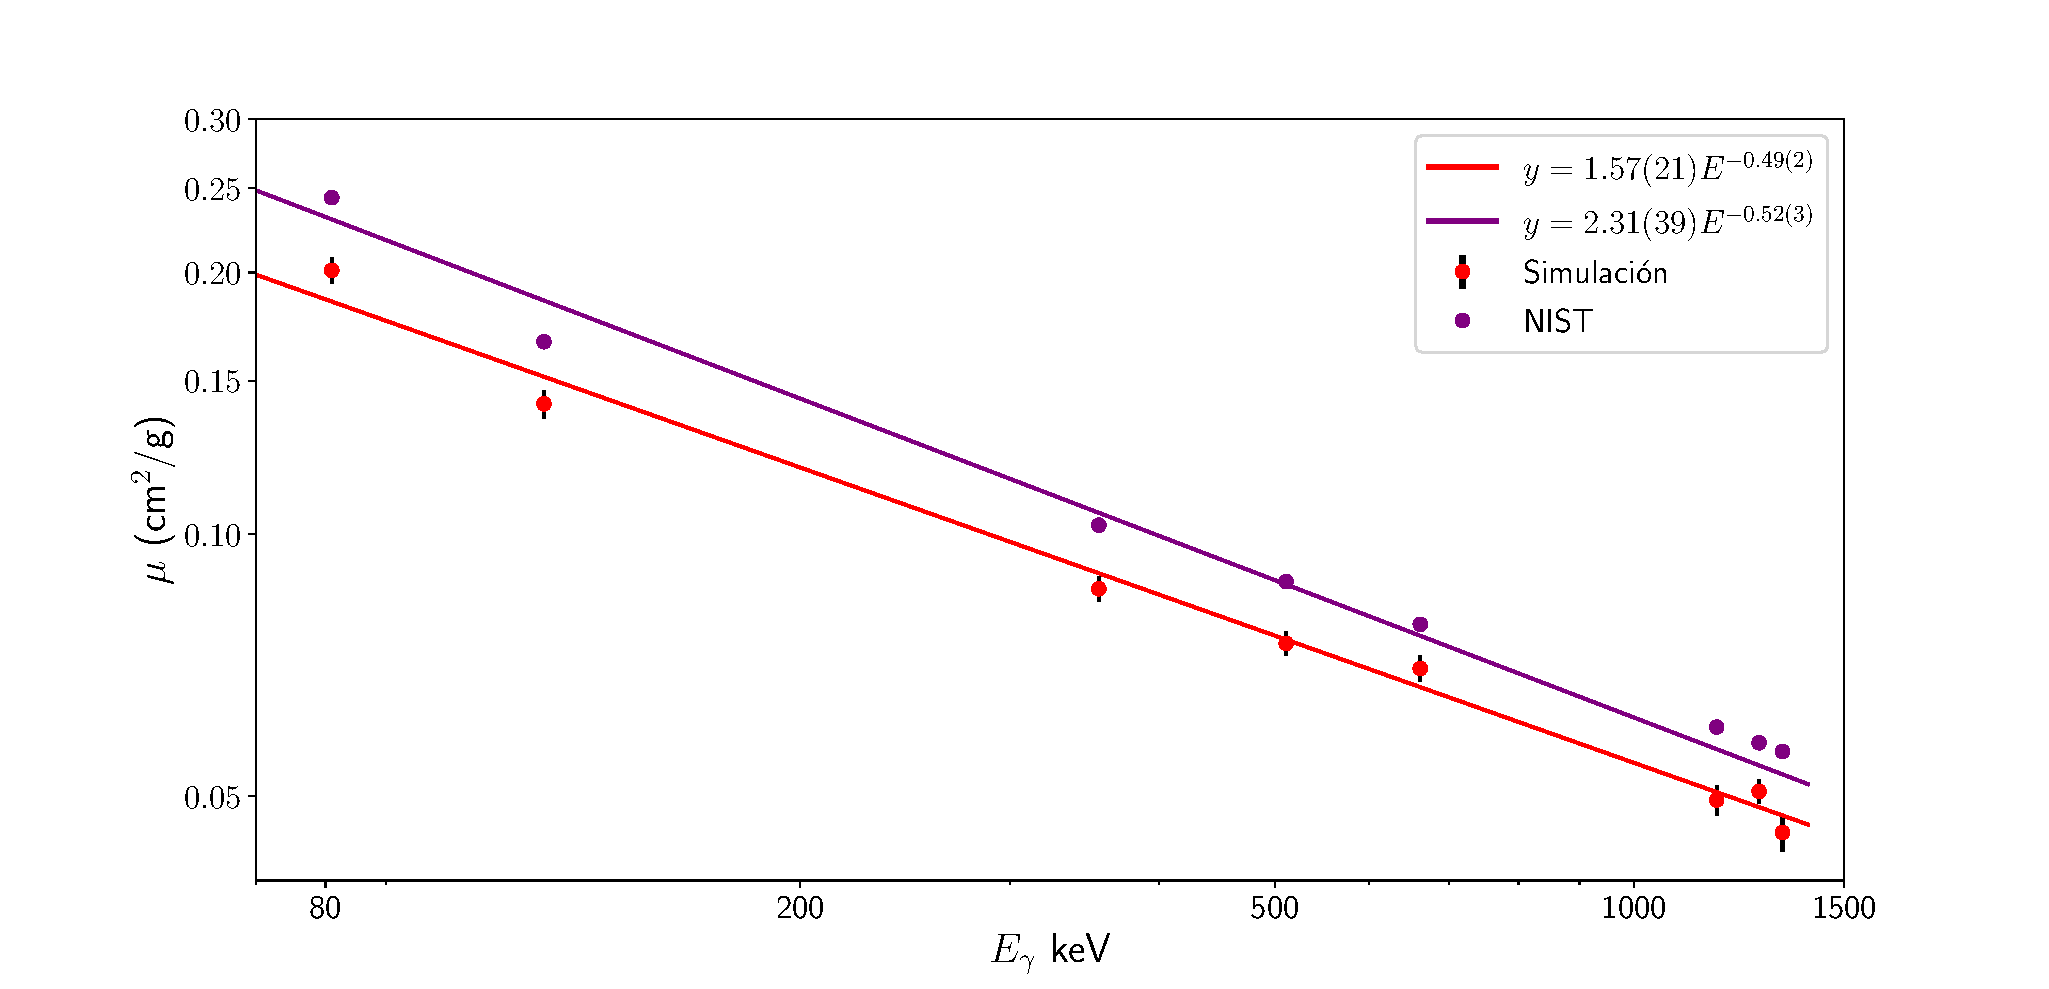
\includegraphics[width=1.0\linewidth]{Kap4/mu-trans-m5.pdf}
	\caption{Ajuste para encontrar $\alpha$ y $n$ a partir de los diferentes $\mu$/$\rho$. Morteros5.}
	\label{fig:mu-trans-m5}
\end{figure}
 
 \subsection{Retrodispersión.}
 
\begin{figure}[H]
	\centering
	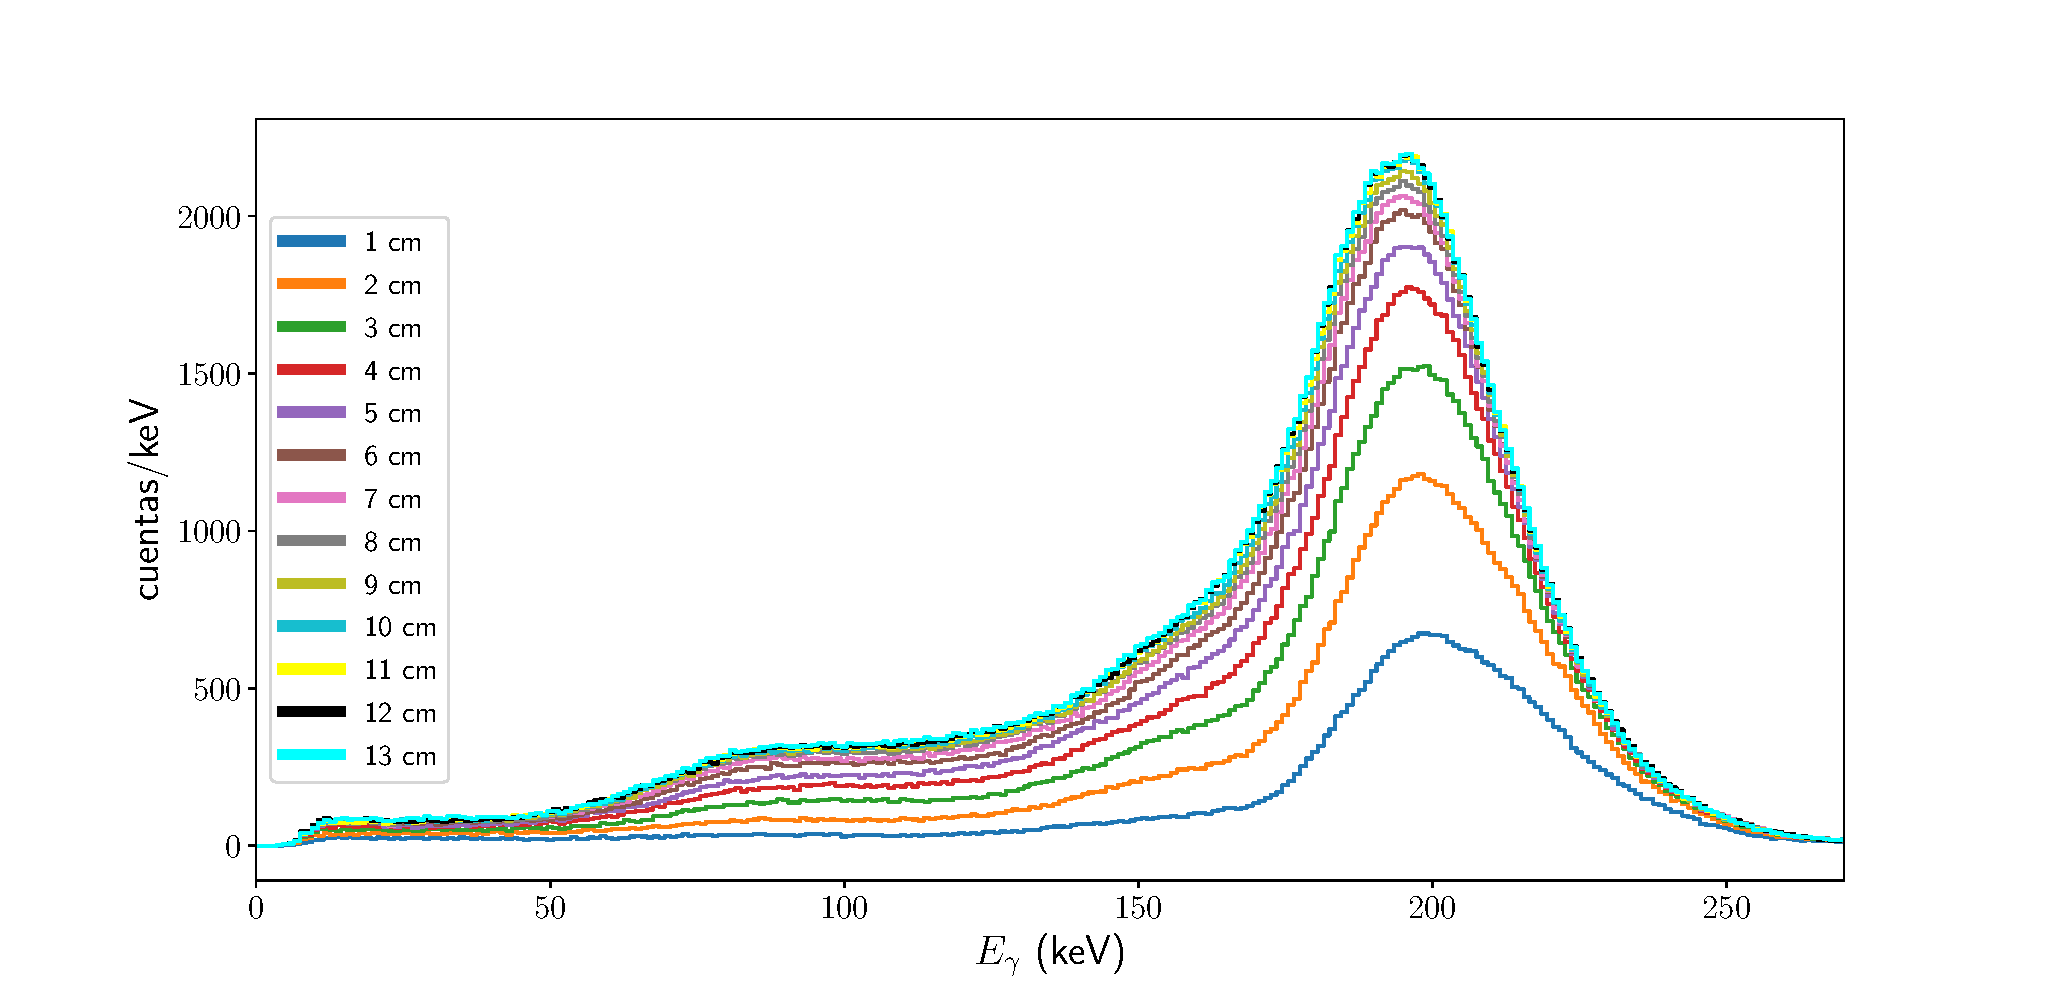
\includegraphics[width=1.0\linewidth]{Kap4/espectro_m5.pdf}
	\caption{Espectro de 10 láminas de Morteros5.}
	\label{fig:espectrom5}
\end{figure}

\begin{figure}[H]
	\centering
	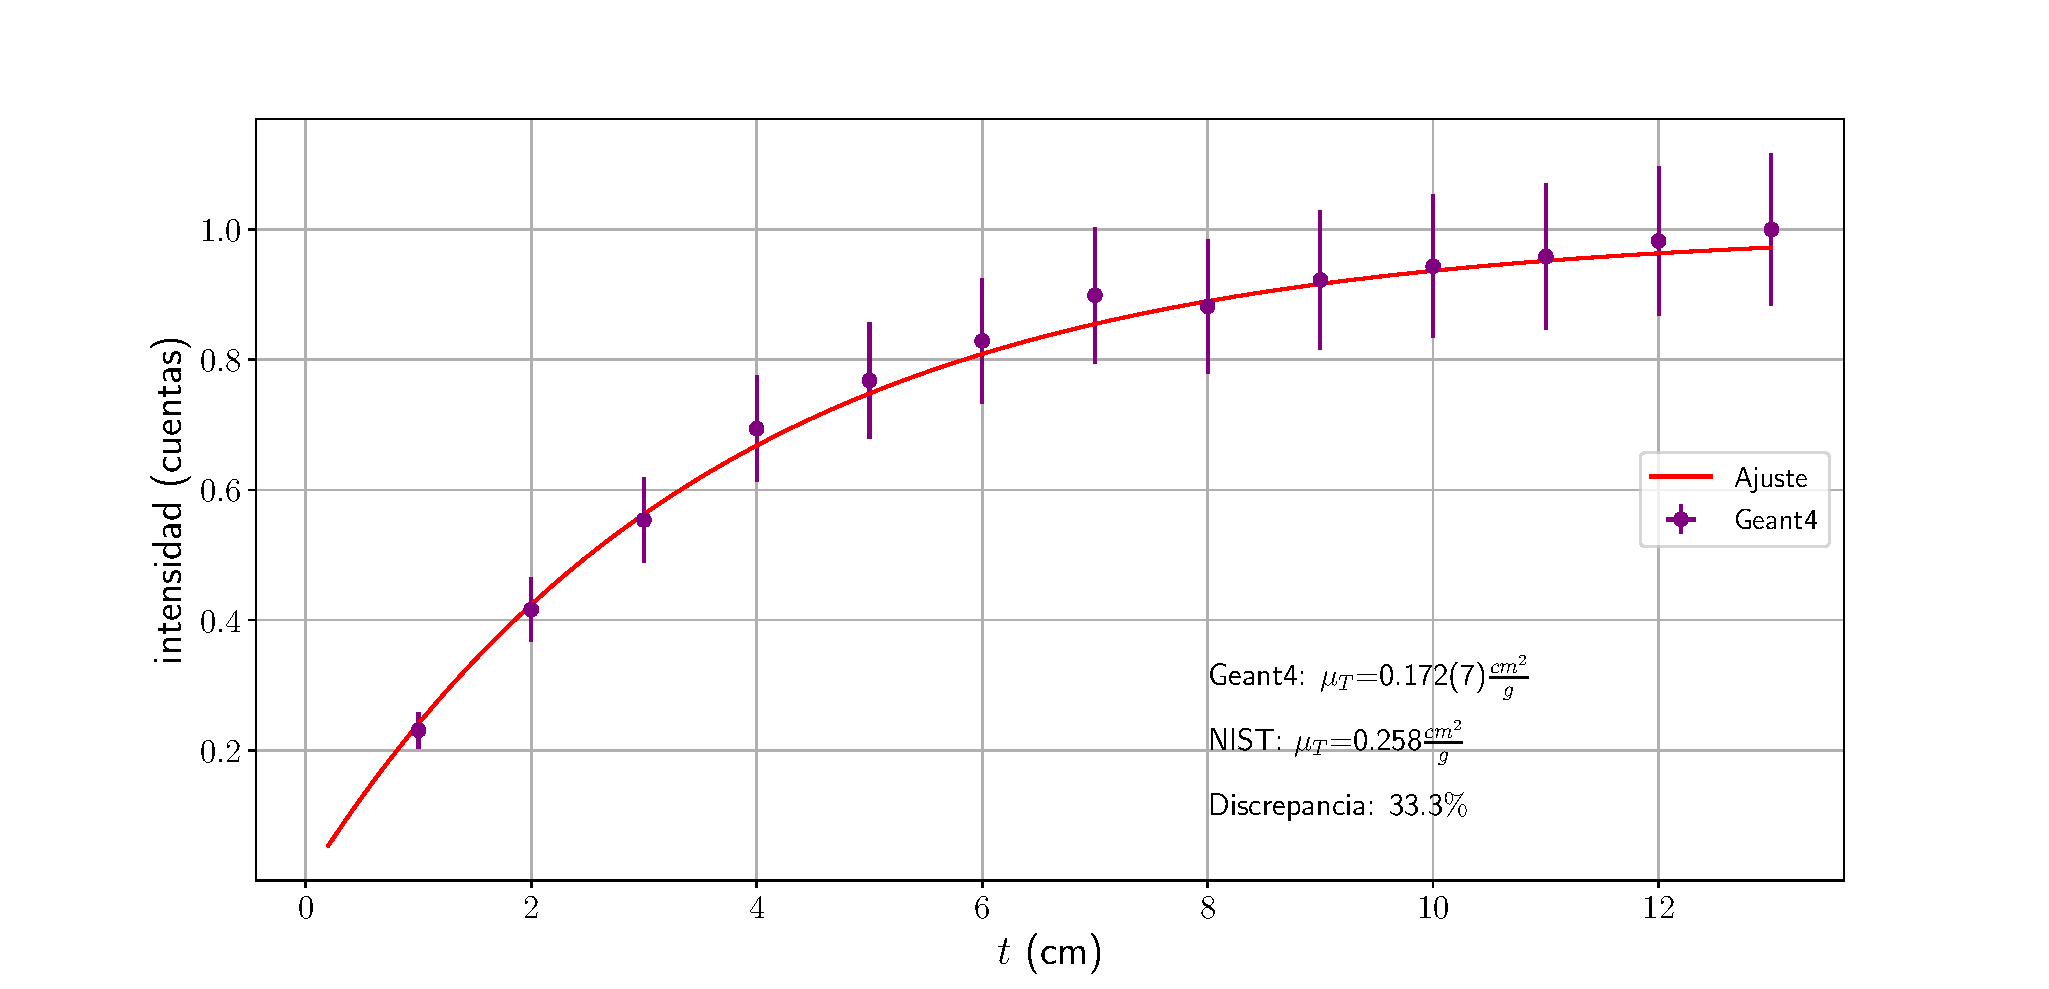
\includegraphics[width=1.0\linewidth]{Kap4/mu_T-m5.pdf}
	\caption{Valores de $\mu_T$. Morteros5.}
	\label{fig:mut-m5}
\end{figure}